\documentclass[twoside]{book}

% Packages required by doxygen
\usepackage{calc}
\usepackage{doxygen}
\usepackage{graphicx}
\usepackage[utf8]{inputenc}
\usepackage{makeidx}
\usepackage{multicol}
\usepackage{multirow}
\usepackage{textcomp}
\usepackage[table]{xcolor}

% Font selection
\usepackage[T1]{fontenc}
\usepackage{mathptmx}
\usepackage[scaled=.90]{helvet}
\usepackage{courier}
\usepackage{amssymb}
\usepackage{sectsty}
\renewcommand{\familydefault}{\sfdefault}
\allsectionsfont{%
  \fontseries{bc}\selectfont%
  \color{darkgray}%
}
\renewcommand{\DoxyLabelFont}{%
  \fontseries{bc}\selectfont%
  \color{darkgray}%
}

% Page & text layout
\usepackage{geometry}
\geometry{%
  a4paper,%
  top=2.5cm,%
  bottom=2.5cm,%
  left=2.5cm,%
  right=2.5cm%
}
\tolerance=750
\hfuzz=15pt
\hbadness=750
\setlength{\emergencystretch}{15pt}
\setlength{\parindent}{0cm}
\setlength{\parskip}{0.2cm}
\makeatletter
\renewcommand{\paragraph}{%
  \@startsection{paragraph}{4}{0ex}{-1.0ex}{1.0ex}{%
    \normalfont\normalsize\bfseries\SS@parafont%
  }%
}
\renewcommand{\subparagraph}{%
  \@startsection{subparagraph}{5}{0ex}{-1.0ex}{1.0ex}{%
    \normalfont\normalsize\bfseries\SS@subparafont%
  }%
}
\makeatother

% Headers & footers
\usepackage{fancyhdr}
\pagestyle{fancyplain}
\fancyhead[LE]{\fancyplain{}{\bfseries\thepage}}
\fancyhead[CE]{\fancyplain{}{}}
\fancyhead[RE]{\fancyplain{}{\bfseries\leftmark}}
\fancyhead[LO]{\fancyplain{}{\bfseries\rightmark}}
\fancyhead[CO]{\fancyplain{}{}}
\fancyhead[RO]{\fancyplain{}{\bfseries\thepage}}
\fancyfoot[LE]{\fancyplain{}{}}
\fancyfoot[CE]{\fancyplain{}{}}
\fancyfoot[RE]{\fancyplain{}{\bfseries\scriptsize Generated on Mon Jan 30 2017 18\-:36\-:17 for Open\-Sky Planetarium by Doxygen }}
\fancyfoot[LO]{\fancyplain{}{\bfseries\scriptsize Generated on Mon Jan 30 2017 18\-:36\-:17 for Open\-Sky Planetarium by Doxygen }}
\fancyfoot[CO]{\fancyplain{}{}}
\fancyfoot[RO]{\fancyplain{}{}}
\renewcommand{\footrulewidth}{0.4pt}
\renewcommand{\chaptermark}[1]{%
  \markboth{#1}{}%
}
\renewcommand{\sectionmark}[1]{%
  \markright{\thesection\ #1}%
}

% Indices & bibliography
\usepackage{natbib}
\usepackage[titles]{tocloft}
\setcounter{tocdepth}{3}
\setcounter{secnumdepth}{5}
\makeindex

% Hyperlinks (required, but should be loaded last)
\usepackage{ifpdf}
\ifpdf
  \usepackage[pdftex,pagebackref=true]{hyperref}
\else
  \usepackage[ps2pdf,pagebackref=true]{hyperref}
\fi
\hypersetup{%
  colorlinks=true,%
  linkcolor=blue,%
  citecolor=blue,%
  unicode%
}

% Custom commands
\newcommand{\clearemptydoublepage}{%
  \newpage{\pagestyle{empty}\cleardoublepage}%
}


%===== C O N T E N T S =====

\begin{document}

% Titlepage & ToC
\hypersetup{pageanchor=false}
\pagenumbering{roman}
\begin{titlepage}
\vspace*{7cm}
\begin{center}%
{\Large Open\-Sky Planetarium }\\
\vspace*{1cm}
{\large Generated by Doxygen 1.8.6}\\
\vspace*{0.5cm}
{\small Mon Jan 30 2017 18:36:17}\\
\end{center}
\end{titlepage}
\clearemptydoublepage
\tableofcontents
\clearemptydoublepage
\pagenumbering{arabic}
\hypersetup{pageanchor=true}

%--- Begin generated contents ---
\chapter{Hierarchical Index}
\section{Class Hierarchy}
This inheritance list is sorted roughly, but not completely, alphabetically\-:\begin{DoxyCompactList}
\item \contentsline{section}{Calibrate}{\pageref{class_calibrate}}{}
\item Q\-Object\begin{DoxyCompactList}
\item \contentsline{section}{Laser\-Dev}{\pageref{class_laser_dev}}{}
\item \contentsline{section}{Open\-Sky\-Planetarium\-Plugin\-Interface}{\pageref{class_open_sky_planetarium_plugin_interface}}{}
\end{DoxyCompactList}
\item Q\-Thread\begin{DoxyCompactList}
\item \contentsline{section}{Serial\-Com}{\pageref{class_serial_com}}{}
\end{DoxyCompactList}
\item Stel\-Dialog\begin{DoxyCompactList}
\item \contentsline{section}{O\-S\-P\-Main\-Dialog}{\pageref{class_o_s_p_main_dialog}}{}
\end{DoxyCompactList}
\item Stel\-Module\begin{DoxyCompactList}
\item \contentsline{section}{Open\-Sky\-Planetarium}{\pageref{class_open_sky_planetarium}}{}
\end{DoxyCompactList}
\item Stel\-Plugin\-Interface\begin{DoxyCompactList}
\item \contentsline{section}{Open\-Sky\-Planetarium\-Plugin\-Interface}{\pageref{class_open_sky_planetarium_plugin_interface}}{}
\end{DoxyCompactList}
\end{DoxyCompactList}

\chapter{Class Index}
\section{Class List}
Here are the classes, structs, unions and interfaces with brief descriptions\-:\begin{DoxyCompactList}
\item\contentsline{section}{\hyperlink{class_calibrate}{Calibrate} \\*Library for coordinates transformations. Calculates the equivalent coordinates between both coordinate systems equatorial and horizontal }{\pageref{class_calibrate}}{}
\item\contentsline{section}{\hyperlink{class_laser_dev}{Laser\-Dev} \\*This class is used for funtions related to motion and turning the laser on and off }{\pageref{class_laser_dev}}{}
\item\contentsline{section}{\hyperlink{class_open_sky_planetarium}{Open\-Sky\-Planetarium} \\*This is used to dynamically load Open Sky Planetarium plugin into stellarium }{\pageref{class_open_sky_planetarium}}{}
\item\contentsline{section}{\hyperlink{class_open_sky_planetarium_plugin_interface}{Open\-Sky\-Planetarium\-Plugin\-Interface} \\*This class is used by Qt to manage a plug-\/in interface }{\pageref{class_open_sky_planetarium_plugin_interface}}{}
\item\contentsline{section}{\hyperlink{class_o_s_p_main_dialog}{O\-S\-P\-Main\-Dialog} \\*This is the main class used in connecting all the signals to gui }{\pageref{class_o_s_p_main_dialog}}{}
\item\contentsline{section}{\hyperlink{class_serial_com}{Serial\-Com} \\*This class is used for funtions related to serial communication with the arduino }{\pageref{class_serial_com}}{}
\end{DoxyCompactList}

\chapter{File Index}
\section{File List}
Here is a list of all files with brief descriptions\-:\begin{DoxyCompactList}
\item\contentsline{section}{\hyperlink{_calibrate_8cpp}{Calibrate.\-cpp} }{\pageref{_calibrate_8cpp}}{}
\item\contentsline{section}{\hyperlink{_calibrate_8hpp}{Calibrate.\-hpp} }{\pageref{_calibrate_8hpp}}{}
\item\contentsline{section}{\hyperlink{_laser_dev_8cpp}{Laser\-Dev.\-cpp} }{\pageref{_laser_dev_8cpp}}{}
\item\contentsline{section}{\hyperlink{_laser_dev_8hpp}{Laser\-Dev.\-hpp} }{\pageref{_laser_dev_8hpp}}{}
\item\contentsline{section}{\hyperlink{_open_sky_planetarium_8cpp}{Open\-Sky\-Planetarium.\-cpp} }{\pageref{_open_sky_planetarium_8cpp}}{}
\item\contentsline{section}{\hyperlink{_open_sky_planetarium_8hpp}{Open\-Sky\-Planetarium.\-hpp} }{\pageref{_open_sky_planetarium_8hpp}}{}
\item\contentsline{section}{\hyperlink{_serial_com_8cpp}{Serial\-Com.\-cpp} }{\pageref{_serial_com_8cpp}}{}
\item\contentsline{section}{\hyperlink{_serial_com_8hpp}{Serial\-Com.\-hpp} }{\pageref{_serial_com_8hpp}}{}
\item\contentsline{section}{gui/\hyperlink{_o_s_p_main_dialog_8cpp}{O\-S\-P\-Main\-Dialog.\-cpp} }{\pageref{_o_s_p_main_dialog_8cpp}}{}
\item\contentsline{section}{gui/\hyperlink{_o_s_p_main_dialog_8hpp}{O\-S\-P\-Main\-Dialog.\-hpp} }{\pageref{_o_s_p_main_dialog_8hpp}}{}
\end{DoxyCompactList}

\chapter{Class Documentation}
\hypertarget{class_calibrate}{\section{Calibrate Class Reference}
\label{class_calibrate}\index{Calibrate@{Calibrate}}
}


Library for coordinates transformations. Calculates the equivalent coordinates between both coordinate systems equatorial and horizontal.  




{\ttfamily \#include $<$Calibrate.\-hpp$>$}

\subsection*{Public Member Functions}
\begin{DoxyCompactItemize}
\item 
\hyperlink{class_calibrate_af7fd8ee2339ee66f6f8e4d9953025796}{Calibrate} ()
\item 
void \hyperlink{class_calibrate_aa995deb89e9bf1afe158a9863feeb9b5}{set\-Time} (double t0)
\item 
void \hyperlink{class_calibrate_accdf063b97064170400a396d50ca364a}{set\-Ref\-\_\-1} (double ar, double dec, double t, double ac, double alt)
\item 
void \hyperlink{class_calibrate_a0de0f875a4426d90c7c67cf9aa7a117c}{set\-Ref\-\_\-2} (double ar, double dec, double t, double ac, double alt)
\item 
void \hyperlink{class_calibrate_af3f3b8373b846d5e19006feef1a29c96}{set\-Ref\-\_\-3} (double ar, double dec, double t, double ac, double alt)
\item 
void \hyperlink{class_calibrate_a21d7622c2356e44897dbfed2f9d9d1d9}{auto\-Ref\-\_\-3} ()
\item 
bool \hyperlink{class_calibrate_a55a935c9efccedcc965cc9de4da5d3be}{is\-Configured} ()
\item 
void \hyperlink{class_calibrate_a611a5a3f616c57325493a4552aadab2c}{get\-H\-Coords} (double ar, double dec, double t, double $\ast$ac, double $\ast$alt)
\item 
void \hyperlink{class_calibrate_ab7e978f3fff297d01addb3decdc2ae15}{get\-E\-Coords} (double ac, double alt, double t, double $\ast$ar, double $\ast$dec)
\end{DoxyCompactItemize}


\subsection{Detailed Description}
Library for coordinates transformations. Calculates the equivalent coordinates between both coordinate systems equatorial and horizontal. 

It's based on Toshimi Taki's matrix method for coordinates transformation\-: \href{http://www.geocities.jp/toshimi_taki/matrix/matrix.htm}{\tt http\-://www.\-geocities.\-jp/toshimi\-\_\-taki/matrix/matrix.\-htm} Contains the necessary methods for setting the initial time, the reference objects, the transformation matrix, and to calculate the equivalent vectors between both coordinate systems. 

Definition at line 36 of file Calibrate.\-hpp.



\subsection{Constructor \& Destructor Documentation}
\hypertarget{class_calibrate_af7fd8ee2339ee66f6f8e4d9953025796}{\index{Calibrate@{Calibrate}!Calibrate@{Calibrate}}
\index{Calibrate@{Calibrate}!Calibrate@{Calibrate}}
\subsubsection[{Calibrate}]{\setlength{\rightskip}{0pt plus 5cm}Calibrate\-::\-Calibrate (
\begin{DoxyParamCaption}
{}
\end{DoxyParamCaption}
)}}\label{class_calibrate_af7fd8ee2339ee66f6f8e4d9953025796}
Class constructor. 

Definition at line 48 of file Calibrate.\-cpp.



\subsection{Member Function Documentation}
\hypertarget{class_calibrate_a21d7622c2356e44897dbfed2f9d9d1d9}{\index{Calibrate@{Calibrate}!auto\-Ref\-\_\-3@{auto\-Ref\-\_\-3}}
\index{auto\-Ref\-\_\-3@{auto\-Ref\-\_\-3}!Calibrate@{Calibrate}}
\subsubsection[{auto\-Ref\-\_\-3}]{\setlength{\rightskip}{0pt plus 5cm}void Calibrate\-::auto\-Ref\-\_\-3 (
\begin{DoxyParamCaption}
{}
\end{DoxyParamCaption}
)}}\label{class_calibrate_a21d7622c2356e44897dbfed2f9d9d1d9}
Third reference object calculated from the two others ones.

Calculates the cross product of the two first reference objects in both coordinates systems, in order to obtain the third one. These two first objects must have 90º from each other, approximately (from 60º to 120º is enough to obtain goods results). 

Definition at line 175 of file Calibrate.\-cpp.

\hypertarget{class_calibrate_ab7e978f3fff297d01addb3decdc2ae15}{\index{Calibrate@{Calibrate}!get\-E\-Coords@{get\-E\-Coords}}
\index{get\-E\-Coords@{get\-E\-Coords}!Calibrate@{Calibrate}}
\subsubsection[{get\-E\-Coords}]{\setlength{\rightskip}{0pt plus 5cm}void Calibrate\-::get\-E\-Coords (
\begin{DoxyParamCaption}
\item[{double}]{ac, }
\item[{double}]{alt, }
\item[{double}]{t, }
\item[{double $\ast$}]{ar, }
\item[{double $\ast$}]{dec}
\end{DoxyParamCaption}
)}}\label{class_calibrate_ab7e978f3fff297d01addb3decdc2ae15}
Equatorial coordinates calculated from the horizontal ones and time.


\begin{DoxyParams}{Parameters}
{\em ac} & Azimuth (horizontal coordinates). \\
\hline
{\em alt} & Altitude (horizontal coordinates). \\
\hline
{\em t} & Unix Timestamp of the Observation. \\
\hline
{\em $\ast$ar} & Pointer to double\-: Returns the right ascension (equatorial coordinates). \\
\hline
{\em $\ast$dec} & Pointer to double\-: Returns the declination (equatorial coordinates). \\
\hline
\end{DoxyParams}


Definition at line 260 of file Calibrate.\-cpp.

\hypertarget{class_calibrate_a611a5a3f616c57325493a4552aadab2c}{\index{Calibrate@{Calibrate}!get\-H\-Coords@{get\-H\-Coords}}
\index{get\-H\-Coords@{get\-H\-Coords}!Calibrate@{Calibrate}}
\subsubsection[{get\-H\-Coords}]{\setlength{\rightskip}{0pt plus 5cm}void Calibrate\-::get\-H\-Coords (
\begin{DoxyParamCaption}
\item[{double}]{ar, }
\item[{double}]{dec, }
\item[{double}]{t, }
\item[{double $\ast$}]{ac, }
\item[{double $\ast$}]{alt}
\end{DoxyParamCaption}
)}}\label{class_calibrate_a611a5a3f616c57325493a4552aadab2c}
Horizontal coordinates calculated from the equatorial ones and time.


\begin{DoxyParams}{Parameters}
{\em ar} & Right Ascension (equatorial coordinates). \\
\hline
{\em dec} & Declination (equatorial coordinates) \\
\hline
{\em t} & Unix Timestamp of the Observation. \\
\hline
{\em $\ast$ac} & Pointer to double\-: Returns the azimuth (horizontal coordiantes). \\
\hline
{\em $\ast$alt} & Pointer to double\-: Returns the altitude (horizontal coordinates). \\
\hline
\end{DoxyParams}


Definition at line 231 of file Calibrate.\-cpp.

\hypertarget{class_calibrate_a55a935c9efccedcc965cc9de4da5d3be}{\index{Calibrate@{Calibrate}!is\-Configured@{is\-Configured}}
\index{is\-Configured@{is\-Configured}!Calibrate@{Calibrate}}
\subsubsection[{is\-Configured}]{\setlength{\rightskip}{0pt plus 5cm}bool Calibrate\-::is\-Configured (
\begin{DoxyParamCaption}
{}
\end{DoxyParamCaption}
)}}\label{class_calibrate_a55a935c9efccedcc965cc9de4da5d3be}
Indicates if the three reference objects has been calculated.

\begin{DoxyReturn}{Returns}
Boolean. 
\end{DoxyReturn}


Definition at line 167 of file Calibrate.\-cpp.

\hypertarget{class_calibrate_accdf063b97064170400a396d50ca364a}{\index{Calibrate@{Calibrate}!set\-Ref\-\_\-1@{set\-Ref\-\_\-1}}
\index{set\-Ref\-\_\-1@{set\-Ref\-\_\-1}!Calibrate@{Calibrate}}
\subsubsection[{set\-Ref\-\_\-1}]{\setlength{\rightskip}{0pt plus 5cm}void Calibrate\-::set\-Ref\-\_\-1 (
\begin{DoxyParamCaption}
\item[{double}]{ar, }
\item[{double}]{dec, }
\item[{double}]{t, }
\item[{double}]{ac, }
\item[{double}]{alt}
\end{DoxyParamCaption}
)}}\label{class_calibrate_accdf063b97064170400a396d50ca364a}
Sets the first reference object from the coordinates in both coordinates systems for that object.


\begin{DoxyParams}{Parameters}
{\em ar} & Right Ascension (equatorial coordinates). \\
\hline
{\em dec} & Declination (equatorial coordinates). \\
\hline
{\em t} & Unix Timestamp of the Observation. \\
\hline
{\em ac} & Azimuth (horizontal coordinates). \\
\hline
{\em alt} & Altitude (horizontal coordinates). \\
\hline
\end{DoxyParams}


Definition at line 127 of file Calibrate.\-cpp.

\hypertarget{class_calibrate_a0de0f875a4426d90c7c67cf9aa7a117c}{\index{Calibrate@{Calibrate}!set\-Ref\-\_\-2@{set\-Ref\-\_\-2}}
\index{set\-Ref\-\_\-2@{set\-Ref\-\_\-2}!Calibrate@{Calibrate}}
\subsubsection[{set\-Ref\-\_\-2}]{\setlength{\rightskip}{0pt plus 5cm}void Calibrate\-::set\-Ref\-\_\-2 (
\begin{DoxyParamCaption}
\item[{double}]{ar, }
\item[{double}]{dec, }
\item[{double}]{t, }
\item[{double}]{ac, }
\item[{double}]{alt}
\end{DoxyParamCaption}
)}}\label{class_calibrate_a0de0f875a4426d90c7c67cf9aa7a117c}
Sets the second reference object from the coordinates in both coordinates systems for that object.


\begin{DoxyParams}{Parameters}
{\em ar} & Right Ascension (equatorial coordinates). \\
\hline
{\em dec} & Declination (equatorial coordinates). \\
\hline
{\em t} & Unix Timestamp of the Observation. \\
\hline
{\em ac} & Azimuth (horizontal coordinates). \\
\hline
{\em alt} & Altitude (horizontal coordinates). \\
\hline
\end{DoxyParams}


Definition at line 141 of file Calibrate.\-cpp.

\hypertarget{class_calibrate_af3f3b8373b846d5e19006feef1a29c96}{\index{Calibrate@{Calibrate}!set\-Ref\-\_\-3@{set\-Ref\-\_\-3}}
\index{set\-Ref\-\_\-3@{set\-Ref\-\_\-3}!Calibrate@{Calibrate}}
\subsubsection[{set\-Ref\-\_\-3}]{\setlength{\rightskip}{0pt plus 5cm}void Calibrate\-::set\-Ref\-\_\-3 (
\begin{DoxyParamCaption}
\item[{double}]{ar, }
\item[{double}]{dec, }
\item[{double}]{t, }
\item[{double}]{ac, }
\item[{double}]{alt}
\end{DoxyParamCaption}
)}}\label{class_calibrate_af3f3b8373b846d5e19006feef1a29c96}
Sets the third reference object from the coordinates in both coordinates systems for that object.


\begin{DoxyParams}{Parameters}
{\em ar} & Right Ascension (equatorial coordinates). \\
\hline
{\em dec} & Declination (equatorial coordinates). \\
\hline
{\em t} & Unix Timestamp of the Observation. \\
\hline
{\em ac} & Azimuth (horizontal coordinates). \\
\hline
{\em alt} & Altitude (horizontal coordinates). \\
\hline
\end{DoxyParams}


Definition at line 155 of file Calibrate.\-cpp.

\hypertarget{class_calibrate_aa995deb89e9bf1afe158a9863feeb9b5}{\index{Calibrate@{Calibrate}!set\-Time@{set\-Time}}
\index{set\-Time@{set\-Time}!Calibrate@{Calibrate}}
\subsubsection[{set\-Time}]{\setlength{\rightskip}{0pt plus 5cm}void Calibrate\-::set\-Time (
\begin{DoxyParamCaption}
\item[{double}]{t0}
\end{DoxyParamCaption}
)}}\label{class_calibrate_aa995deb89e9bf1afe158a9863feeb9b5}
Sets the initial time.

This parameter is used in order to consider time passing on horizontal coordinates system.


\begin{DoxyParams}{Parameters}
{\em t0} & Unix Timestamp of the initial observation time. \\
\hline
\end{DoxyParams}


Definition at line 119 of file Calibrate.\-cpp.



The documentation for this class was generated from the following files\-:\begin{DoxyCompactItemize}
\item 
\hyperlink{_calibrate_8hpp}{Calibrate.\-hpp}\item 
\hyperlink{_calibrate_8cpp}{Calibrate.\-cpp}\end{DoxyCompactItemize}

\hypertarget{class_laser_dev}{\section{Laser\-Dev Class Reference}
\label{class_laser_dev}\index{Laser\-Dev@{Laser\-Dev}}
}


This class is used for funtions related to motion and turning the laser on and off.  




{\ttfamily \#include $<$Laser\-Dev.\-hpp$>$}

Inheritance diagram for Laser\-Dev\-:\begin{figure}[H]
\begin{center}
\leavevmode
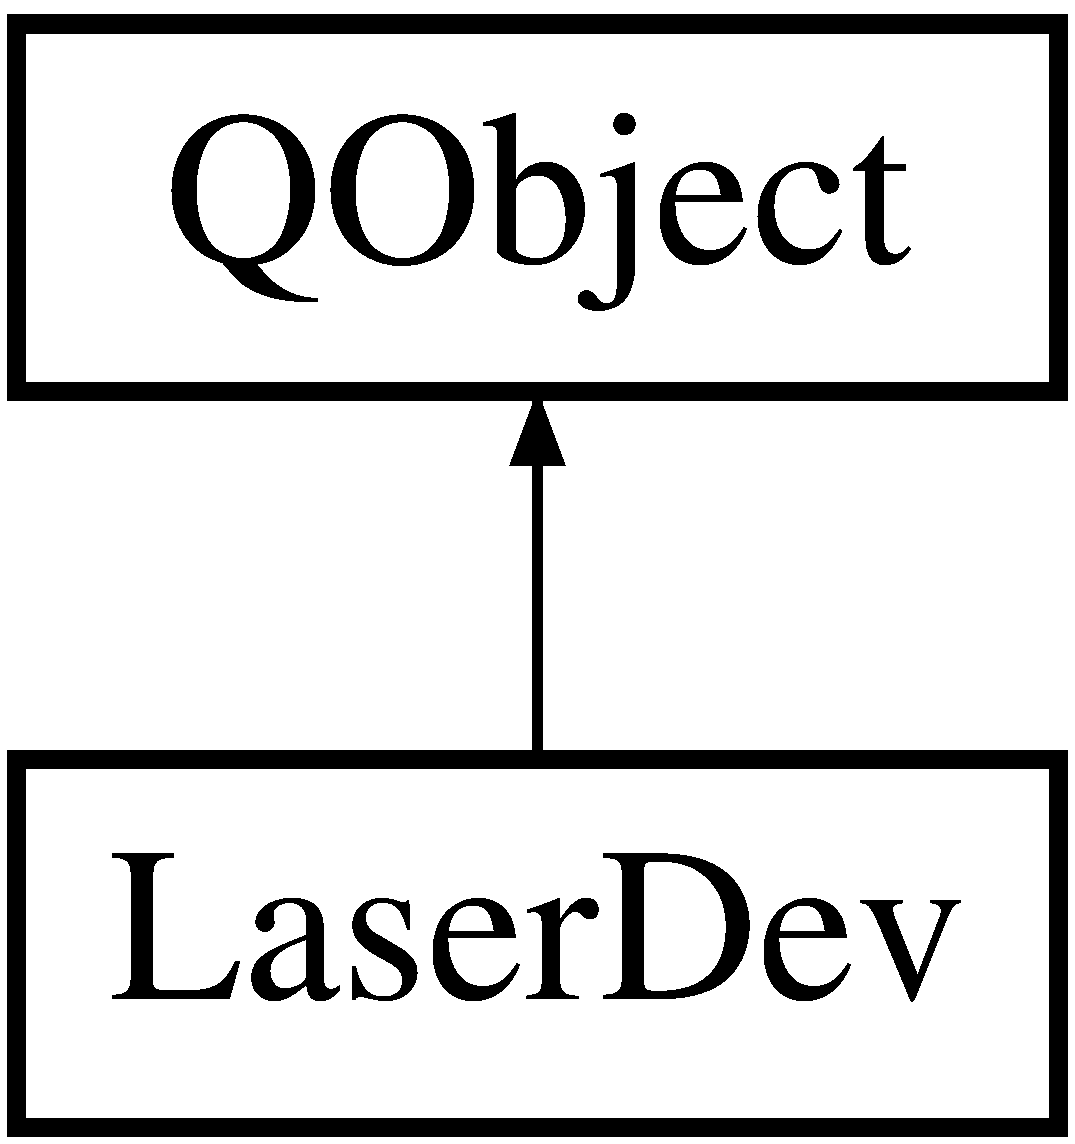
\includegraphics[height=2.000000cm]{class_laser_dev}
\end{center}
\end{figure}
\subsection*{Public Slots}
\begin{DoxyCompactItemize}
\item 
void \hyperlink{class_laser_dev_acafc5e4275cf1fab74218af7af7f34e5}{get\-Pos} ()
\item 
void \hyperlink{class_laser_dev_a337541ffca93b0c2900778a91554ede6}{process\-Error} (const Q\-String \&s)
\item 
void \hyperlink{class_laser_dev_ab016d27d125aa27c856b281e2f9e5370}{process\-Timeout} (const Q\-String \&s)
\item 
void \hyperlink{class_laser_dev_a527679c655073b74703b7399a1adbe8d}{sread} (const Q\-String \&s)
\item 
void \hyperlink{class_laser_dev_aedb2ff8257a72247202b5434780a1655}{init} ()
\item 
void \hyperlink{class_laser_dev_ae66064fa79825cfdc8fb604db0d462af}{move} (double x, double y)
\item 
void \hyperlink{class_laser_dev_a2e229a59571fa9dcd93ebc6a23ecb3c1}{movx} (int sign\-Dir)
\item 
void \hyperlink{class_laser_dev_a6d9a60d963031c9104200014a380b55e}{movy} (int sign\-Dir)
\item 
void \hyperlink{class_laser_dev_a06c0022d17589088dfc7a0dcc56141ed}{stop} ()
\item 
void \hyperlink{class_laser_dev_aee2527432d2b36107c42f3307c8f8c47}{laser\-On} ()
\item 
void \hyperlink{class_laser_dev_a19059c3f944c0c0dae17485676fea678}{laser\-Off} ()
\end{DoxyCompactItemize}
\subsection*{Signals}
\begin{DoxyCompactItemize}
\item 
void \hyperlink{class_laser_dev_a5f64ad8bfee8c6a870d5b6cf8c22ad85}{debug\-\_\-send} (Q\-String s)
\item 
void \hyperlink{class_laser_dev_a6e1ab7df7165fdf0a2df02a1a2e459ae}{pos\-\_\-received} (Q\-String, Q\-String)
\end{DoxyCompactItemize}
\subsection*{Public Member Functions}
\begin{DoxyCompactItemize}
\item 
\hyperlink{class_laser_dev_a9d9aa26eac4043fd9674856745b228ea}{Laser\-Dev} (Q\-Object $\ast$parent=0)
\item 
\hyperlink{class_laser_dev_a8b57b80183af8eaa9611a9b6cae3d635}{$\sim$\-Laser\-Dev} ()
\item 
void \hyperlink{class_laser_dev_af33d1e8b41f8f14b451f59cf2d491512}{set\-Port\-Name} (const Q\-String \&s)
\end{DoxyCompactItemize}


\subsection{Detailed Description}
This class is used for funtions related to motion and turning the laser on and off. 

Definition at line 32 of file Laser\-Dev.\-hpp.



\subsection{Constructor \& Destructor Documentation}
\hypertarget{class_laser_dev_a9d9aa26eac4043fd9674856745b228ea}{\index{Laser\-Dev@{Laser\-Dev}!Laser\-Dev@{Laser\-Dev}}
\index{Laser\-Dev@{Laser\-Dev}!LaserDev@{Laser\-Dev}}
\subsubsection[{Laser\-Dev}]{\setlength{\rightskip}{0pt plus 5cm}Laser\-Dev\-::\-Laser\-Dev (
\begin{DoxyParamCaption}
\item[{Q\-Object $\ast$}]{parent = {\ttfamily 0}}
\end{DoxyParamCaption}
)}}\label{class_laser_dev_a9d9aa26eac4043fd9674856745b228ea}
Class constructor. 

Definition at line 35 of file Laser\-Dev.\-cpp.

\hypertarget{class_laser_dev_a8b57b80183af8eaa9611a9b6cae3d635}{\index{Laser\-Dev@{Laser\-Dev}!$\sim$\-Laser\-Dev@{$\sim$\-Laser\-Dev}}
\index{$\sim$\-Laser\-Dev@{$\sim$\-Laser\-Dev}!LaserDev@{Laser\-Dev}}
\subsubsection[{$\sim$\-Laser\-Dev}]{\setlength{\rightskip}{0pt plus 5cm}Laser\-Dev\-::$\sim$\-Laser\-Dev (
\begin{DoxyParamCaption}
{}
\end{DoxyParamCaption}
)}}\label{class_laser_dev_a8b57b80183af8eaa9611a9b6cae3d635}
Class destructor. 

Definition at line 48 of file Laser\-Dev.\-cpp.



\subsection{Member Function Documentation}
\hypertarget{class_laser_dev_a5f64ad8bfee8c6a870d5b6cf8c22ad85}{\index{Laser\-Dev@{Laser\-Dev}!debug\-\_\-send@{debug\-\_\-send}}
\index{debug\-\_\-send@{debug\-\_\-send}!LaserDev@{Laser\-Dev}}
\subsubsection[{debug\-\_\-send}]{\setlength{\rightskip}{0pt plus 5cm}void Laser\-Dev\-::debug\-\_\-send (
\begin{DoxyParamCaption}
\item[{Q\-String}]{s}
\end{DoxyParamCaption}
)\hspace{0.3cm}{\ttfamily [signal]}}}\label{class_laser_dev_a5f64ad8bfee8c6a870d5b6cf8c22ad85}
Sending the debug signal \hypertarget{class_laser_dev_acafc5e4275cf1fab74218af7af7f34e5}{\index{Laser\-Dev@{Laser\-Dev}!get\-Pos@{get\-Pos}}
\index{get\-Pos@{get\-Pos}!LaserDev@{Laser\-Dev}}
\subsubsection[{get\-Pos}]{\setlength{\rightskip}{0pt plus 5cm}void Laser\-Dev\-::get\-Pos (
\begin{DoxyParamCaption}
{}
\end{DoxyParamCaption}
)\hspace{0.3cm}{\ttfamily [slot]}}}\label{class_laser_dev_acafc5e4275cf1fab74218af7af7f34e5}
This function is called to get the current position of the telescope in radians 

Definition at line 151 of file Laser\-Dev.\-cpp.

\hypertarget{class_laser_dev_aedb2ff8257a72247202b5434780a1655}{\index{Laser\-Dev@{Laser\-Dev}!init@{init}}
\index{init@{init}!LaserDev@{Laser\-Dev}}
\subsubsection[{init}]{\setlength{\rightskip}{0pt plus 5cm}void Laser\-Dev\-::init (
\begin{DoxyParamCaption}
{}
\end{DoxyParamCaption}
)\hspace{0.3cm}{\ttfamily [slot]}}}\label{class_laser_dev_aedb2ff8257a72247202b5434780a1655}
sends the \char`\"{}init\char`\"{} command to the device and after \char`\"{}done\-\_\-init\char`\"{} is received from the device, emits \char`\"{}init\-\_\-received\char`\"{} signal 

Definition at line 141 of file Laser\-Dev.\-cpp.

\hypertarget{class_laser_dev_a19059c3f944c0c0dae17485676fea678}{\index{Laser\-Dev@{Laser\-Dev}!laser\-Off@{laser\-Off}}
\index{laser\-Off@{laser\-Off}!LaserDev@{Laser\-Dev}}
\subsubsection[{laser\-Off}]{\setlength{\rightskip}{0pt plus 5cm}void Laser\-Dev\-::laser\-Off (
\begin{DoxyParamCaption}
{}
\end{DoxyParamCaption}
)\hspace{0.3cm}{\ttfamily [slot]}}}\label{class_laser_dev_a19059c3f944c0c0dae17485676fea678}
To turn the laser off 

Definition at line 222 of file Laser\-Dev.\-cpp.

\hypertarget{class_laser_dev_aee2527432d2b36107c42f3307c8f8c47}{\index{Laser\-Dev@{Laser\-Dev}!laser\-On@{laser\-On}}
\index{laser\-On@{laser\-On}!LaserDev@{Laser\-Dev}}
\subsubsection[{laser\-On}]{\setlength{\rightskip}{0pt plus 5cm}void Laser\-Dev\-::laser\-On (
\begin{DoxyParamCaption}
{}
\end{DoxyParamCaption}
)\hspace{0.3cm}{\ttfamily [slot]}}}\label{class_laser_dev_aee2527432d2b36107c42f3307c8f8c47}
to turn the laser on 

Definition at line 212 of file Laser\-Dev.\-cpp.

\hypertarget{class_laser_dev_ae66064fa79825cfdc8fb604db0d462af}{\index{Laser\-Dev@{Laser\-Dev}!move@{move}}
\index{move@{move}!LaserDev@{Laser\-Dev}}
\subsubsection[{move}]{\setlength{\rightskip}{0pt plus 5cm}void Laser\-Dev\-::move (
\begin{DoxyParamCaption}
\item[{double}]{x, }
\item[{double}]{y}
\end{DoxyParamCaption}
)\hspace{0.3cm}{\ttfamily [slot]}}}\label{class_laser_dev_ae66064fa79825cfdc8fb604db0d462af}
Sends the telescope coordinates to the device 
\begin{DoxyParams}{Parameters}
{\em x} & Azimuth fed to arduino. \\
\hline
{\em y} & Altitude fed to arduino. \\
\hline
\end{DoxyParams}


Definition at line 162 of file Laser\-Dev.\-cpp.

\hypertarget{class_laser_dev_a2e229a59571fa9dcd93ebc6a23ecb3c1}{\index{Laser\-Dev@{Laser\-Dev}!movx@{movx}}
\index{movx@{movx}!LaserDev@{Laser\-Dev}}
\subsubsection[{movx}]{\setlength{\rightskip}{0pt plus 5cm}void Laser\-Dev\-::movx (
\begin{DoxyParamCaption}
\item[{int}]{sign\-Dir}
\end{DoxyParamCaption}
)\hspace{0.3cm}{\ttfamily [slot]}}}\label{class_laser_dev_a2e229a59571fa9dcd93ebc6a23ecb3c1}
To move the laser in x direction depending on sign\-Dir 

Definition at line 191 of file Laser\-Dev.\-cpp.

\hypertarget{class_laser_dev_a6d9a60d963031c9104200014a380b55e}{\index{Laser\-Dev@{Laser\-Dev}!movy@{movy}}
\index{movy@{movy}!LaserDev@{Laser\-Dev}}
\subsubsection[{movy}]{\setlength{\rightskip}{0pt plus 5cm}void Laser\-Dev\-::movy (
\begin{DoxyParamCaption}
\item[{int}]{sign\-Dir}
\end{DoxyParamCaption}
)\hspace{0.3cm}{\ttfamily [slot]}}}\label{class_laser_dev_a6d9a60d963031c9104200014a380b55e}
To move the laser in y direction depending on sign\-Dir /param sign\-Dir 0 to move up 1 to move down 

Definition at line 178 of file Laser\-Dev.\-cpp.

\hypertarget{class_laser_dev_a6e1ab7df7165fdf0a2df02a1a2e459ae}{\index{Laser\-Dev@{Laser\-Dev}!pos\-\_\-received@{pos\-\_\-received}}
\index{pos\-\_\-received@{pos\-\_\-received}!LaserDev@{Laser\-Dev}}
\subsubsection[{pos\-\_\-received}]{\setlength{\rightskip}{0pt plus 5cm}void Laser\-Dev\-::pos\-\_\-received (
\begin{DoxyParamCaption}
\item[{Q\-String}]{, }
\item[{Q\-String}]{}
\end{DoxyParamCaption}
)\hspace{0.3cm}{\ttfamily [signal]}}}\label{class_laser_dev_a6e1ab7df7165fdf0a2df02a1a2e459ae}
Recieving the position from arduino \hypertarget{class_laser_dev_a337541ffca93b0c2900778a91554ede6}{\index{Laser\-Dev@{Laser\-Dev}!process\-Error@{process\-Error}}
\index{process\-Error@{process\-Error}!LaserDev@{Laser\-Dev}}
\subsubsection[{process\-Error}]{\setlength{\rightskip}{0pt plus 5cm}void Laser\-Dev\-::process\-Error (
\begin{DoxyParamCaption}
\item[{const Q\-String \&}]{s}
\end{DoxyParamCaption}
)\hspace{0.3cm}{\ttfamily [slot]}}}\label{class_laser_dev_a337541ffca93b0c2900778a91554ede6}
slot for the error, sends the signal to \hyperlink{class_o_s_p_main_dialog}{O\-S\-P\-Main\-Dialog} 

Definition at line 56 of file Laser\-Dev.\-cpp.

\hypertarget{class_laser_dev_ab016d27d125aa27c856b281e2f9e5370}{\index{Laser\-Dev@{Laser\-Dev}!process\-Timeout@{process\-Timeout}}
\index{process\-Timeout@{process\-Timeout}!LaserDev@{Laser\-Dev}}
\subsubsection[{process\-Timeout}]{\setlength{\rightskip}{0pt plus 5cm}void Laser\-Dev\-::process\-Timeout (
\begin{DoxyParamCaption}
\item[{const Q\-String \&}]{s}
\end{DoxyParamCaption}
)\hspace{0.3cm}{\ttfamily [slot]}}}\label{class_laser_dev_ab016d27d125aa27c856b281e2f9e5370}
slot for the timeout , sends the signal to \hyperlink{class_o_s_p_main_dialog}{O\-S\-P\-Main\-Dialog} 

Definition at line 63 of file Laser\-Dev.\-cpp.

\hypertarget{class_laser_dev_af33d1e8b41f8f14b451f59cf2d491512}{\index{Laser\-Dev@{Laser\-Dev}!set\-Port\-Name@{set\-Port\-Name}}
\index{set\-Port\-Name@{set\-Port\-Name}!LaserDev@{Laser\-Dev}}
\subsubsection[{set\-Port\-Name}]{\setlength{\rightskip}{0pt plus 5cm}void Laser\-Dev\-::set\-Port\-Name (
\begin{DoxyParamCaption}
\item[{const Q\-String \&}]{s}
\end{DoxyParamCaption}
)}}\label{class_laser_dev_af33d1e8b41f8f14b451f59cf2d491512}
function for setting the port\-Name 
\begin{DoxyParams}{Parameters}
{\em s} & port name \\
\hline
\end{DoxyParams}


Definition at line 71 of file Laser\-Dev.\-cpp.

\hypertarget{class_laser_dev_a527679c655073b74703b7399a1adbe8d}{\index{Laser\-Dev@{Laser\-Dev}!sread@{sread}}
\index{sread@{sread}!LaserDev@{Laser\-Dev}}
\subsubsection[{sread}]{\setlength{\rightskip}{0pt plus 5cm}void Laser\-Dev\-::sread (
\begin{DoxyParamCaption}
\item[{const Q\-String \&}]{s}
\end{DoxyParamCaption}
)\hspace{0.3cm}{\ttfamily [slot]}}}\label{class_laser_dev_a527679c655073b74703b7399a1adbe8d}
This function is called after writing to the serial port. This function performs various steps like echo\-Data, get\-Steps, get\-Horizontal\-Coords, get\-Vertical\-Coords 

Definition at line 81 of file Laser\-Dev.\-cpp.

\hypertarget{class_laser_dev_a06c0022d17589088dfc7a0dcc56141ed}{\index{Laser\-Dev@{Laser\-Dev}!stop@{stop}}
\index{stop@{stop}!LaserDev@{Laser\-Dev}}
\subsubsection[{stop}]{\setlength{\rightskip}{0pt plus 5cm}void Laser\-Dev\-::stop (
\begin{DoxyParamCaption}
{}
\end{DoxyParamCaption}
)\hspace{0.3cm}{\ttfamily [slot]}}}\label{class_laser_dev_a06c0022d17589088dfc7a0dcc56141ed}
to stop the laser movements in either of the direction x or y /param sign\-Dir 0 to move up 1 to move down 

Definition at line 203 of file Laser\-Dev.\-cpp.



The documentation for this class was generated from the following files\-:\begin{DoxyCompactItemize}
\item 
\hyperlink{_laser_dev_8hpp}{Laser\-Dev.\-hpp}\item 
\hyperlink{_laser_dev_8cpp}{Laser\-Dev.\-cpp}\end{DoxyCompactItemize}

\hypertarget{class_open_sky_planetarium}{\section{Open\-Sky\-Planetarium Class Reference}
\label{class_open_sky_planetarium}\index{Open\-Sky\-Planetarium@{Open\-Sky\-Planetarium}}
}


This is used to dynamically load Open Sky Planetarium plugin into stellarium.  




{\ttfamily \#include $<$Open\-Sky\-Planetarium.\-hpp$>$}

Inheritance diagram for Open\-Sky\-Planetarium\-:\begin{figure}[H]
\begin{center}
\leavevmode
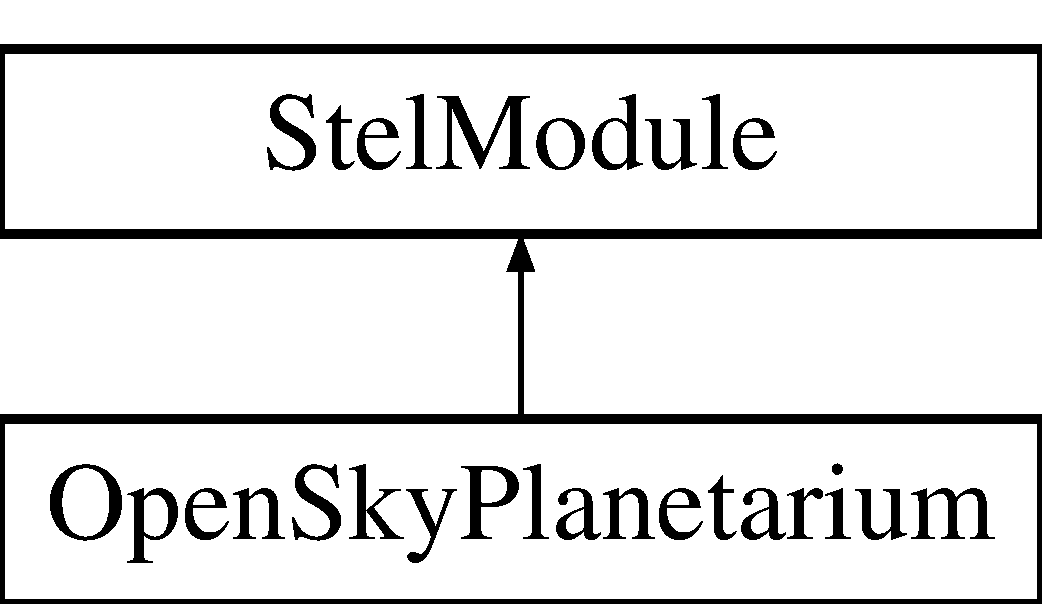
\includegraphics[height=2.000000cm]{class_open_sky_planetarium}
\end{center}
\end{figure}
\subsection*{Public Member Functions}
\begin{DoxyCompactItemize}
\item 
\hyperlink{class_open_sky_planetarium_a5f8863f2909ea7c84722d8f1d1410aac}{Open\-Sky\-Planetarium} ()
\item 
\hyperlink{class_open_sky_planetarium_a4df59ddbb670aef575f97bbcef1267c8}{$\sim$\-Open\-Sky\-Planetarium} ()
\item 
virtual void \hyperlink{class_open_sky_planetarium_ad3219ba7597f58f41eb2f175b5b3ca43}{init} ()
\item 
virtual void \hyperlink{class_open_sky_planetarium_a163cb7c2ecf113d829f0eec67d4e853d}{deinit} ()
\item 
virtual void \hyperlink{class_open_sky_planetarium_a71cdbeed316e46fc4e84bf76fadabe62}{update} (double)
\item 
virtual double \hyperlink{class_open_sky_planetarium_a7880a253b939c93cc93bb10bbc04fd96}{get\-Call\-Order} (Stel\-Module\-Action\-Name action\-Name) const 
\item 
virtual bool \hyperlink{class_open_sky_planetarium_a36c4660bffbd77013a7f1007f9cace16}{configure\-Gui} (bool show)
\end{DoxyCompactItemize}


\subsection{Detailed Description}
This is used to dynamically load Open Sky Planetarium plugin into stellarium. 

Definition at line 30 of file Open\-Sky\-Planetarium.\-hpp.



\subsection{Constructor \& Destructor Documentation}
\hypertarget{class_open_sky_planetarium_a5f8863f2909ea7c84722d8f1d1410aac}{\index{Open\-Sky\-Planetarium@{Open\-Sky\-Planetarium}!Open\-Sky\-Planetarium@{Open\-Sky\-Planetarium}}
\index{Open\-Sky\-Planetarium@{Open\-Sky\-Planetarium}!OpenSkyPlanetarium@{Open\-Sky\-Planetarium}}
\subsubsection[{Open\-Sky\-Planetarium}]{\setlength{\rightskip}{0pt plus 5cm}Open\-Sky\-Planetarium\-::\-Open\-Sky\-Planetarium (
\begin{DoxyParamCaption}
{}
\end{DoxyParamCaption}
)}}\label{class_open_sky_planetarium_a5f8863f2909ea7c84722d8f1d1410aac}
Class constructor. 

Definition at line 60 of file Open\-Sky\-Planetarium.\-cpp.

\hypertarget{class_open_sky_planetarium_a4df59ddbb670aef575f97bbcef1267c8}{\index{Open\-Sky\-Planetarium@{Open\-Sky\-Planetarium}!$\sim$\-Open\-Sky\-Planetarium@{$\sim$\-Open\-Sky\-Planetarium}}
\index{$\sim$\-Open\-Sky\-Planetarium@{$\sim$\-Open\-Sky\-Planetarium}!OpenSkyPlanetarium@{Open\-Sky\-Planetarium}}
\subsubsection[{$\sim$\-Open\-Sky\-Planetarium}]{\setlength{\rightskip}{0pt plus 5cm}Open\-Sky\-Planetarium\-::$\sim$\-Open\-Sky\-Planetarium (
\begin{DoxyParamCaption}
{}
\end{DoxyParamCaption}
)}}\label{class_open_sky_planetarium_a4df59ddbb670aef575f97bbcef1267c8}
Class destructor. 

Definition at line 69 of file Open\-Sky\-Planetarium.\-cpp.



\subsection{Member Function Documentation}
\hypertarget{class_open_sky_planetarium_a36c4660bffbd77013a7f1007f9cace16}{\index{Open\-Sky\-Planetarium@{Open\-Sky\-Planetarium}!configure\-Gui@{configure\-Gui}}
\index{configure\-Gui@{configure\-Gui}!OpenSkyPlanetarium@{Open\-Sky\-Planetarium}}
\subsubsection[{configure\-Gui}]{\setlength{\rightskip}{0pt plus 5cm}bool Open\-Sky\-Planetarium\-::configure\-Gui (
\begin{DoxyParamCaption}
\item[{bool}]{show}
\end{DoxyParamCaption}
)\hspace{0.3cm}{\ttfamily [virtual]}}}\label{class_open_sky_planetarium_a36c4660bffbd77013a7f1007f9cace16}
This method is used to show the plugin interface 

Definition at line 86 of file Open\-Sky\-Planetarium.\-cpp.

\hypertarget{class_open_sky_planetarium_a163cb7c2ecf113d829f0eec67d4e853d}{\index{Open\-Sky\-Planetarium@{Open\-Sky\-Planetarium}!deinit@{deinit}}
\index{deinit@{deinit}!OpenSkyPlanetarium@{Open\-Sky\-Planetarium}}
\subsubsection[{deinit}]{\setlength{\rightskip}{0pt plus 5cm}void Open\-Sky\-Planetarium\-::deinit (
\begin{DoxyParamCaption}
{}
\end{DoxyParamCaption}
)\hspace{0.3cm}{\ttfamily [virtual]}}}\label{class_open_sky_planetarium_a163cb7c2ecf113d829f0eec67d4e853d}
This method is used to delete the instance of main Window 

Definition at line 122 of file Open\-Sky\-Planetarium.\-cpp.

\hypertarget{class_open_sky_planetarium_a7880a253b939c93cc93bb10bbc04fd96}{\index{Open\-Sky\-Planetarium@{Open\-Sky\-Planetarium}!get\-Call\-Order@{get\-Call\-Order}}
\index{get\-Call\-Order@{get\-Call\-Order}!OpenSkyPlanetarium@{Open\-Sky\-Planetarium}}
\subsubsection[{get\-Call\-Order}]{\setlength{\rightskip}{0pt plus 5cm}double Open\-Sky\-Planetarium\-::get\-Call\-Order (
\begin{DoxyParamCaption}
\item[{Stel\-Module\-Action\-Name}]{action\-Name}
\end{DoxyParamCaption}
) const\hspace{0.3cm}{\ttfamily [virtual]}}}\label{class_open_sky_planetarium_a7880a253b939c93cc93bb10bbc04fd96}
This method is used to reimplement the get\-Call\-Order method 

Definition at line 76 of file Open\-Sky\-Planetarium.\-cpp.

\hypertarget{class_open_sky_planetarium_ad3219ba7597f58f41eb2f175b5b3ca43}{\index{Open\-Sky\-Planetarium@{Open\-Sky\-Planetarium}!init@{init}}
\index{init@{init}!OpenSkyPlanetarium@{Open\-Sky\-Planetarium}}
\subsubsection[{init}]{\setlength{\rightskip}{0pt plus 5cm}void Open\-Sky\-Planetarium\-::init (
\begin{DoxyParamCaption}
{}
\end{DoxyParamCaption}
)\hspace{0.3cm}{\ttfamily [virtual]}}}\label{class_open_sky_planetarium_ad3219ba7597f58f41eb2f175b5b3ca43}
Init Open Sky Planetarium module 

Definition at line 94 of file Open\-Sky\-Planetarium.\-cpp.

\hypertarget{class_open_sky_planetarium_a71cdbeed316e46fc4e84bf76fadabe62}{\index{Open\-Sky\-Planetarium@{Open\-Sky\-Planetarium}!update@{update}}
\index{update@{update}!OpenSkyPlanetarium@{Open\-Sky\-Planetarium}}
\subsubsection[{update}]{\setlength{\rightskip}{0pt plus 5cm}virtual void Open\-Sky\-Planetarium\-::update (
\begin{DoxyParamCaption}
\item[{double}]{}
\end{DoxyParamCaption}
)\hspace{0.3cm}{\ttfamily [inline]}, {\ttfamily [virtual]}}}\label{class_open_sky_planetarium_a71cdbeed316e46fc4e84bf76fadabe62}


Definition at line 57 of file Open\-Sky\-Planetarium.\-hpp.



The documentation for this class was generated from the following files\-:\begin{DoxyCompactItemize}
\item 
\hyperlink{_open_sky_planetarium_8hpp}{Open\-Sky\-Planetarium.\-hpp}\item 
\hyperlink{_open_sky_planetarium_8cpp}{Open\-Sky\-Planetarium.\-cpp}\end{DoxyCompactItemize}

\hypertarget{class_open_sky_planetarium_plugin_interface}{\section{Open\-Sky\-Planetarium\-Plugin\-Interface Class Reference}
\label{class_open_sky_planetarium_plugin_interface}\index{Open\-Sky\-Planetarium\-Plugin\-Interface@{Open\-Sky\-Planetarium\-Plugin\-Interface}}
}


This class is used by Qt to manage a plug-\/in interface.  




{\ttfamily \#include $<$Open\-Sky\-Planetarium.\-hpp$>$}

Inheritance diagram for Open\-Sky\-Planetarium\-Plugin\-Interface\-:\begin{figure}[H]
\begin{center}
\leavevmode
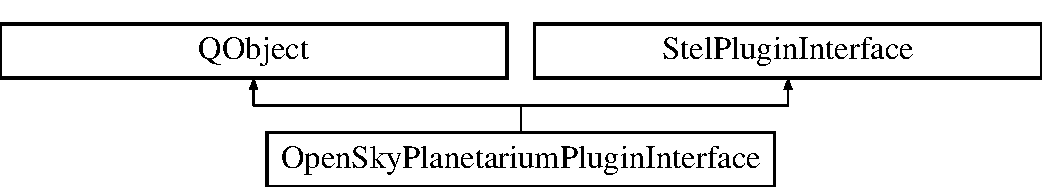
\includegraphics[height=2.000000cm]{class_open_sky_planetarium_plugin_interface}
\end{center}
\end{figure}
\subsection*{Public Member Functions}
\begin{DoxyCompactItemize}
\item 
virtual Stel\-Module $\ast$ \hyperlink{class_open_sky_planetarium_plugin_interface_af89d90ab4d905c0818ca6bdc966ed6ee}{get\-Stel\-Module} () const 
\item 
virtual Stel\-Plugin\-Info \hyperlink{class_open_sky_planetarium_plugin_interface_afb592a06233f9bea5e6149e7bfd364aa}{get\-Plugin\-Info} () const 
\end{DoxyCompactItemize}


\subsection{Detailed Description}
This class is used by Qt to manage a plug-\/in interface. 

Definition at line 79 of file Open\-Sky\-Planetarium.\-hpp.



\subsection{Member Function Documentation}
\hypertarget{class_open_sky_planetarium_plugin_interface_afb592a06233f9bea5e6149e7bfd364aa}{\index{Open\-Sky\-Planetarium\-Plugin\-Interface@{Open\-Sky\-Planetarium\-Plugin\-Interface}!get\-Plugin\-Info@{get\-Plugin\-Info}}
\index{get\-Plugin\-Info@{get\-Plugin\-Info}!OpenSkyPlanetariumPluginInterface@{Open\-Sky\-Planetarium\-Plugin\-Interface}}
\subsubsection[{get\-Plugin\-Info}]{\setlength{\rightskip}{0pt plus 5cm}Stel\-Plugin\-Info Open\-Sky\-Planetarium\-Plugin\-Interface\-::get\-Plugin\-Info (
\begin{DoxyParamCaption}
{}
\end{DoxyParamCaption}
) const\hspace{0.3cm}{\ttfamily [virtual]}}}\label{class_open_sky_planetarium_plugin_interface_afb592a06233f9bea5e6149e7bfd364aa}
This method is used to pass the information about the Open\-Sky Planetarium plugin. 

Definition at line 43 of file Open\-Sky\-Planetarium.\-cpp.

\hypertarget{class_open_sky_planetarium_plugin_interface_af89d90ab4d905c0818ca6bdc966ed6ee}{\index{Open\-Sky\-Planetarium\-Plugin\-Interface@{Open\-Sky\-Planetarium\-Plugin\-Interface}!get\-Stel\-Module@{get\-Stel\-Module}}
\index{get\-Stel\-Module@{get\-Stel\-Module}!OpenSkyPlanetariumPluginInterface@{Open\-Sky\-Planetarium\-Plugin\-Interface}}
\subsubsection[{get\-Stel\-Module}]{\setlength{\rightskip}{0pt plus 5cm}Stel\-Module $\ast$ Open\-Sky\-Planetarium\-Plugin\-Interface\-::get\-Stel\-Module (
\begin{DoxyParamCaption}
{}
\end{DoxyParamCaption}
) const\hspace{0.3cm}{\ttfamily [virtual]}}}\label{class_open_sky_planetarium_plugin_interface_af89d90ab4d905c0818ca6bdc966ed6ee}
This method is the one called automatically by the Stel\-Module\-Mgr just after loading the dynamic library 

Definition at line 38 of file Open\-Sky\-Planetarium.\-cpp.



The documentation for this class was generated from the following files\-:\begin{DoxyCompactItemize}
\item 
\hyperlink{_open_sky_planetarium_8hpp}{Open\-Sky\-Planetarium.\-hpp}\item 
\hyperlink{_open_sky_planetarium_8cpp}{Open\-Sky\-Planetarium.\-cpp}\end{DoxyCompactItemize}

\hypertarget{class_o_s_p_main_dialog}{\section{O\-S\-P\-Main\-Dialog Class Reference}
\label{class_o_s_p_main_dialog}\index{O\-S\-P\-Main\-Dialog@{O\-S\-P\-Main\-Dialog}}
}


This is the main class used in connecting all the signals to gui.  




{\ttfamily \#include $<$O\-S\-P\-Main\-Dialog.\-hpp$>$}

Inheritance diagram for O\-S\-P\-Main\-Dialog\-:\begin{figure}[H]
\begin{center}
\leavevmode
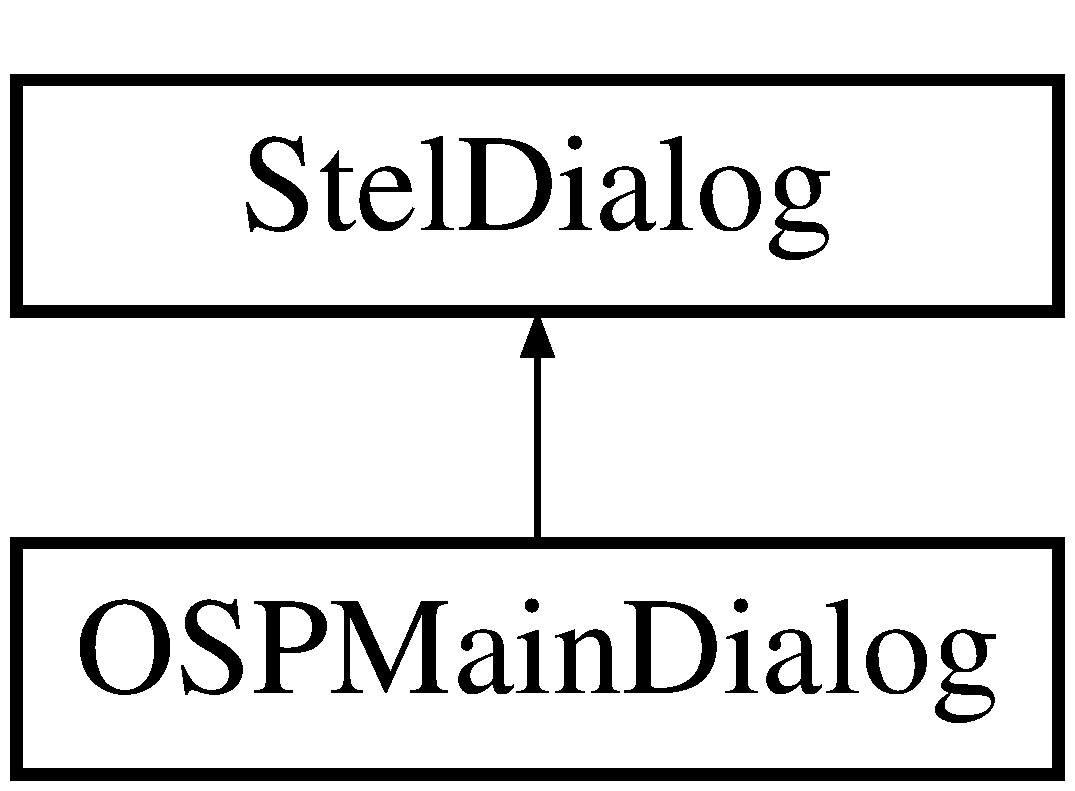
\includegraphics[height=2.000000cm]{class_o_s_p_main_dialog}
\end{center}
\end{figure}
\subsection*{Public Slots}
\begin{DoxyCompactItemize}
\item 
void \hyperlink{class_o_s_p_main_dialog_a47ea6fd9f98519cc31e72f5de34a9306}{retranslate} ()
\item 
void \hyperlink{class_o_s_p_main_dialog_a3e1eb9ec4e4b720c5710b6dd919cff2a}{debug\-\_\-received} (Q\-String s)
\item 
void \hyperlink{class_o_s_p_main_dialog_af8d49ae6630b09271fe3f3eecf083e75}{pos\-\_\-received} (Q\-String x, Q\-String y)
\item 
void \hyperlink{class_o_s_p_main_dialog_a4ef91ba4a5c2de748ae3863108f64ed1}{select\-Device} ()
\item 
void \hyperlink{class_o_s_p_main_dialog_ab70551cf5084beb1a448070784224b5e}{init\-Device} ()
\item 
void \hyperlink{class_o_s_p_main_dialog_a8d977df774af144d6b587874dc72bb6d}{arrow\-\_\-released} ()
\item 
void \hyperlink{class_o_s_p_main_dialog_a1d029fbbacb738ec5f96387afc4a148c}{up\-Pressed} ()
\item 
void \hyperlink{class_o_s_p_main_dialog_a2d9c9e8eadf0566c6a62b56c256d3036}{down\-Pressed} ()
\item 
void \hyperlink{class_o_s_p_main_dialog_add7447fb9aa1e92241e9dafb24be9eee}{right\-Pressed} ()
\item 
void \hyperlink{class_o_s_p_main_dialog_a53254f5a2f14008f0b28e599055db78c}{left\-Pressed} ()
\item 
void \hyperlink{class_o_s_p_main_dialog_a50277876272e2b18f4feaed7147805cb}{laser\-Toggled} ()
\item 
void \hyperlink{class_o_s_p_main_dialog_a440099805a95258b244578f44797b2fb}{set\-Reference} ()
\item 
void \hyperlink{class_o_s_p_main_dialog_a7f89737ac4e508e1149950f5ca3f62f7}{go\-To} ()
\item 
void \hyperlink{class_o_s_p_main_dialog_a81e34e4b686fc8a240b8b60fce8db716}{open\-Script} ()
\item 
void \hyperlink{class_o_s_p_main_dialog_a3a2279d534043892ce314ebd3676a946}{save\-Script} ()
\item 
void \hyperlink{class_o_s_p_main_dialog_a82deaf58658ee7df200d4c3ead6dc238}{exec\-Script} ()
\item 
void \hyperlink{class_o_s_p_main_dialog_a147004f47bd6872358d2a1503394df43}{compile\-Script} ()
\item 
void \hyperlink{class_o_s_p_main_dialog_a0dc634b74f2f1e2a0fcf3e948e46b761}{laser} (bool stat)
\item 
void \hyperlink{class_o_s_p_main_dialog_ad3fec79d0def25964f5adab237abf682}{play\-Audio} (Q\-String fname)
\item 
void \hyperlink{class_o_s_p_main_dialog_ad59f47b89d0a2d70d6ec56829069641d}{waitforsec} (int min, int sec)
\item 
void \hyperlink{class_o_s_p_main_dialog_a926b0132bfacc026a35847ec0c1f8b0a}{move} (Q\-String, Q\-String)
\item 
void \hyperlink{class_o_s_p_main_dialog_aab37bcc54ff79d3bf3a1442b3fa27072}{gt} ()
\item 
void \hyperlink{class_o_s_p_main_dialog_a30be772a3ccc49a2e06ce3417f2f2d5c}{pl} ()
\item 
void \hyperlink{class_o_s_p_main_dialog_accc6706706a6606f941b913cd9e6bdb6}{lo} ()
\item 
void \hyperlink{class_o_s_p_main_dialog_a8f6b102204eb71c786ddc3d05e80601e}{wt} ()
\item 
void \hyperlink{class_o_s_p_main_dialog_ab8473d80b4c5220361b55d310c033858}{set\-Volume} (int volume)
\item 
void \hyperlink{class_o_s_p_main_dialog_a2427cbbbec577cd4df51f5a993a74bf8}{play\-Clicked} ()
\item 
void \hyperlink{class_o_s_p_main_dialog_a5781ec6f0fa33cea8174fcaf335664af}{stop\-Click} ()
\end{DoxyCompactItemize}
\subsection*{Signals}
\begin{DoxyCompactItemize}
\item 
void \hyperlink{class_o_s_p_main_dialog_a35e47dd2960e4a5b1ca07ce11a806432}{com\-G\-O\-T\-O} (Q\-String sra, Q\-String sdec)
\item 
void \hyperlink{class_o_s_p_main_dialog_a5b5dea4eef55d376856d4cfd7eba92f3}{com\-T\-U\-R\-N} (bool stat)
\item 
void \hyperlink{class_o_s_p_main_dialog_a761b06593a36f1830a009ca4f644c859}{com\-W\-A\-I\-T} (int min, int sec)
\item 
void \hyperlink{class_o_s_p_main_dialog_a022dc536831ad2fa62b3935ff64d977e}{com\-P\-L\-A\-Y} (Q\-String fname)
\item 
void \hyperlink{class_o_s_p_main_dialog_a42763b78bcbcb452a8c8054de364f6fc}{play} ()
\item 
void \hyperlink{class_o_s_p_main_dialog_aa1e618f2fe9cb6253b9a783faf34f6c7}{pause} ()
\item 
void \hyperlink{class_o_s_p_main_dialog_a53f55236a4ab1d0569fc8b2be4a3753e}{stop} ()
\end{DoxyCompactItemize}
\subsection*{Public Member Functions}
\begin{DoxyCompactItemize}
\item 
\hyperlink{class_o_s_p_main_dialog_a10db9ace40cfdd733c99d1fa9564bd2a}{O\-S\-P\-Main\-Dialog} ()
\item 
\hyperlink{class_o_s_p_main_dialog_a56031e057b554531243afdeeee57a811}{$\sim$\-O\-S\-P\-Main\-Dialog} ()
\item 
void \hyperlink{class_o_s_p_main_dialog_a9ed0230ee9b9aca9d377cbe489b8cc05}{set\-Signals} ()
\item 
void \hyperlink{class_o_s_p_main_dialog_ace2c5f32c8ec0512f8bcb972f5350e5f}{show\-Message} (Q\-String m)
\end{DoxyCompactItemize}
\subsection*{Protected Member Functions}
\begin{DoxyCompactItemize}
\item 
void \hyperlink{class_o_s_p_main_dialog_a57985a48791e4fbfd747a7d7e14ec4ca}{create\-Dialog\-Content} ()
\end{DoxyCompactItemize}


\subsection{Detailed Description}
This is the main class used in connecting all the signals to gui. 

Definition at line 39 of file O\-S\-P\-Main\-Dialog.\-hpp.



\subsection{Constructor \& Destructor Documentation}
\hypertarget{class_o_s_p_main_dialog_a10db9ace40cfdd733c99d1fa9564bd2a}{\index{O\-S\-P\-Main\-Dialog@{O\-S\-P\-Main\-Dialog}!O\-S\-P\-Main\-Dialog@{O\-S\-P\-Main\-Dialog}}
\index{O\-S\-P\-Main\-Dialog@{O\-S\-P\-Main\-Dialog}!OSPMainDialog@{O\-S\-P\-Main\-Dialog}}
\subsubsection[{O\-S\-P\-Main\-Dialog}]{\setlength{\rightskip}{0pt plus 5cm}O\-S\-P\-Main\-Dialog\-::\-O\-S\-P\-Main\-Dialog (
\begin{DoxyParamCaption}
{}
\end{DoxyParamCaption}
)}}\label{class_o_s_p_main_dialog_a10db9ace40cfdd733c99d1fa9564bd2a}


Definition at line 50 of file O\-S\-P\-Main\-Dialog.\-cpp.

\hypertarget{class_o_s_p_main_dialog_a56031e057b554531243afdeeee57a811}{\index{O\-S\-P\-Main\-Dialog@{O\-S\-P\-Main\-Dialog}!$\sim$\-O\-S\-P\-Main\-Dialog@{$\sim$\-O\-S\-P\-Main\-Dialog}}
\index{$\sim$\-O\-S\-P\-Main\-Dialog@{$\sim$\-O\-S\-P\-Main\-Dialog}!OSPMainDialog@{O\-S\-P\-Main\-Dialog}}
\subsubsection[{$\sim$\-O\-S\-P\-Main\-Dialog}]{\setlength{\rightskip}{0pt plus 5cm}O\-S\-P\-Main\-Dialog\-::$\sim$\-O\-S\-P\-Main\-Dialog (
\begin{DoxyParamCaption}
{}
\end{DoxyParamCaption}
)}}\label{class_o_s_p_main_dialog_a56031e057b554531243afdeeee57a811}


Definition at line 78 of file O\-S\-P\-Main\-Dialog.\-cpp.



\subsection{Member Function Documentation}
\hypertarget{class_o_s_p_main_dialog_a8d977df774af144d6b587874dc72bb6d}{\index{O\-S\-P\-Main\-Dialog@{O\-S\-P\-Main\-Dialog}!arrow\-\_\-released@{arrow\-\_\-released}}
\index{arrow\-\_\-released@{arrow\-\_\-released}!OSPMainDialog@{O\-S\-P\-Main\-Dialog}}
\subsubsection[{arrow\-\_\-released}]{\setlength{\rightskip}{0pt plus 5cm}void O\-S\-P\-Main\-Dialog\-::arrow\-\_\-released (
\begin{DoxyParamCaption}
{}
\end{DoxyParamCaption}
)\hspace{0.3cm}{\ttfamily [slot]}}}\label{class_o_s_p_main_dialog_a8d977df774af144d6b587874dc72bb6d}
This function is called when the Up(mv\-Up), Down(mv\-Down), Right(mv\-Right) and Left(mv\-Left) button is released This function sends the stop command to the arduino device to stop its movement along any of the four directions 

Definition at line 273 of file O\-S\-P\-Main\-Dialog.\-cpp.

\hypertarget{class_o_s_p_main_dialog_a35e47dd2960e4a5b1ca07ce11a806432}{\index{O\-S\-P\-Main\-Dialog@{O\-S\-P\-Main\-Dialog}!com\-G\-O\-T\-O@{com\-G\-O\-T\-O}}
\index{com\-G\-O\-T\-O@{com\-G\-O\-T\-O}!OSPMainDialog@{O\-S\-P\-Main\-Dialog}}
\subsubsection[{com\-G\-O\-T\-O}]{\setlength{\rightskip}{0pt plus 5cm}void O\-S\-P\-Main\-Dialog\-::com\-G\-O\-T\-O (
\begin{DoxyParamCaption}
\item[{Q\-String}]{sra, }
\item[{Q\-String}]{sdec}
\end{DoxyParamCaption}
)\hspace{0.3cm}{\ttfamily [signal]}}}\label{class_o_s_p_main_dialog_a35e47dd2960e4a5b1ca07ce11a806432}
This signal is connected to move of \hyperlink{class_o_s_p_main_dialog}{O\-S\-P\-Main\-Dialog} class 
\begin{DoxyParams}{Parameters}
{\em sra} & Right Ascension (equatorial coordinates). \\
\hline
{\em dec} & Declination (equatorial coordinates). \\
\hline
\end{DoxyParams}
\hypertarget{class_o_s_p_main_dialog_a147004f47bd6872358d2a1503394df43}{\index{O\-S\-P\-Main\-Dialog@{O\-S\-P\-Main\-Dialog}!compile\-Script@{compile\-Script}}
\index{compile\-Script@{compile\-Script}!OSPMainDialog@{O\-S\-P\-Main\-Dialog}}
\subsubsection[{compile\-Script}]{\setlength{\rightskip}{0pt plus 5cm}void O\-S\-P\-Main\-Dialog\-::compile\-Script (
\begin{DoxyParamCaption}
{}
\end{DoxyParamCaption}
)\hspace{0.3cm}{\ttfamily [slot]}}}\label{class_o_s_p_main_dialog_a147004f47bd6872358d2a1503394df43}
This function is used to compile script. This function maps the user script commands to the C++ functions 

Definition at line 447 of file O\-S\-P\-Main\-Dialog.\-cpp.

\hypertarget{class_o_s_p_main_dialog_a022dc536831ad2fa62b3935ff64d977e}{\index{O\-S\-P\-Main\-Dialog@{O\-S\-P\-Main\-Dialog}!com\-P\-L\-A\-Y@{com\-P\-L\-A\-Y}}
\index{com\-P\-L\-A\-Y@{com\-P\-L\-A\-Y}!OSPMainDialog@{O\-S\-P\-Main\-Dialog}}
\subsubsection[{com\-P\-L\-A\-Y}]{\setlength{\rightskip}{0pt plus 5cm}void O\-S\-P\-Main\-Dialog\-::com\-P\-L\-A\-Y (
\begin{DoxyParamCaption}
\item[{Q\-String}]{fname}
\end{DoxyParamCaption}
)\hspace{0.3cm}{\ttfamily [signal]}}}\label{class_o_s_p_main_dialog_a022dc536831ad2fa62b3935ff64d977e}
This signal is connected to play\-Audio of \hyperlink{class_o_s_p_main_dialog}{O\-S\-P\-Main\-Dialog} class 
\begin{DoxyParams}{Parameters}
{\em fname} & file name \\
\hline
\end{DoxyParams}
\hypertarget{class_o_s_p_main_dialog_a5b5dea4eef55d376856d4cfd7eba92f3}{\index{O\-S\-P\-Main\-Dialog@{O\-S\-P\-Main\-Dialog}!com\-T\-U\-R\-N@{com\-T\-U\-R\-N}}
\index{com\-T\-U\-R\-N@{com\-T\-U\-R\-N}!OSPMainDialog@{O\-S\-P\-Main\-Dialog}}
\subsubsection[{com\-T\-U\-R\-N}]{\setlength{\rightskip}{0pt plus 5cm}void O\-S\-P\-Main\-Dialog\-::com\-T\-U\-R\-N (
\begin{DoxyParamCaption}
\item[{bool}]{stat}
\end{DoxyParamCaption}
)\hspace{0.3cm}{\ttfamily [signal]}}}\label{class_o_s_p_main_dialog_a5b5dea4eef55d376856d4cfd7eba92f3}
This signal is connected to laser of \hyperlink{class_o_s_p_main_dialog}{O\-S\-P\-Main\-Dialog} class 
\begin{DoxyParams}{Parameters}
{\em stat} & status of laser \\
\hline
\end{DoxyParams}
\hypertarget{class_o_s_p_main_dialog_a761b06593a36f1830a009ca4f644c859}{\index{O\-S\-P\-Main\-Dialog@{O\-S\-P\-Main\-Dialog}!com\-W\-A\-I\-T@{com\-W\-A\-I\-T}}
\index{com\-W\-A\-I\-T@{com\-W\-A\-I\-T}!OSPMainDialog@{O\-S\-P\-Main\-Dialog}}
\subsubsection[{com\-W\-A\-I\-T}]{\setlength{\rightskip}{0pt plus 5cm}void O\-S\-P\-Main\-Dialog\-::com\-W\-A\-I\-T (
\begin{DoxyParamCaption}
\item[{int}]{min, }
\item[{int}]{sec}
\end{DoxyParamCaption}
)\hspace{0.3cm}{\ttfamily [signal]}}}\label{class_o_s_p_main_dialog_a761b06593a36f1830a009ca4f644c859}
This signal is connected to waitforsec of \hyperlink{class_o_s_p_main_dialog}{O\-S\-P\-Main\-Dialog} class 
\begin{DoxyParams}{Parameters}
{\em min} & time in minute \\
\hline
{\em sec} & time in second \\
\hline
\end{DoxyParams}
\hypertarget{class_o_s_p_main_dialog_a57985a48791e4fbfd747a7d7e14ec4ca}{\index{O\-S\-P\-Main\-Dialog@{O\-S\-P\-Main\-Dialog}!create\-Dialog\-Content@{create\-Dialog\-Content}}
\index{create\-Dialog\-Content@{create\-Dialog\-Content}!OSPMainDialog@{O\-S\-P\-Main\-Dialog}}
\subsubsection[{create\-Dialog\-Content}]{\setlength{\rightskip}{0pt plus 5cm}void O\-S\-P\-Main\-Dialog\-::create\-Dialog\-Content (
\begin{DoxyParamCaption}
{}
\end{DoxyParamCaption}
)\hspace{0.3cm}{\ttfamily [protected]}}}\label{class_o_s_p_main_dialog_a57985a48791e4fbfd747a7d7e14ec4ca}
This function is used to create a dialog box and set the current index of the box 

Definition at line 92 of file O\-S\-P\-Main\-Dialog.\-cpp.

\hypertarget{class_o_s_p_main_dialog_a3e1eb9ec4e4b720c5710b6dd919cff2a}{\index{O\-S\-P\-Main\-Dialog@{O\-S\-P\-Main\-Dialog}!debug\-\_\-received@{debug\-\_\-received}}
\index{debug\-\_\-received@{debug\-\_\-received}!OSPMainDialog@{O\-S\-P\-Main\-Dialog}}
\subsubsection[{debug\-\_\-received}]{\setlength{\rightskip}{0pt plus 5cm}void O\-S\-P\-Main\-Dialog\-::debug\-\_\-received (
\begin{DoxyParamCaption}
\item[{Q\-String}]{s}
\end{DoxyParamCaption}
)\hspace{0.3cm}{\ttfamily [slot]}}}\label{class_o_s_p_main_dialog_a3e1eb9ec4e4b720c5710b6dd919cff2a}
This funtion is connected to many signals for debugging purpose. 
\begin{DoxyParams}{Parameters}
{\em s} & Debug string \\
\hline
\end{DoxyParams}


Definition at line 173 of file O\-S\-P\-Main\-Dialog.\-cpp.

\hypertarget{class_o_s_p_main_dialog_a2d9c9e8eadf0566c6a62b56c256d3036}{\index{O\-S\-P\-Main\-Dialog@{O\-S\-P\-Main\-Dialog}!down\-Pressed@{down\-Pressed}}
\index{down\-Pressed@{down\-Pressed}!OSPMainDialog@{O\-S\-P\-Main\-Dialog}}
\subsubsection[{down\-Pressed}]{\setlength{\rightskip}{0pt plus 5cm}void O\-S\-P\-Main\-Dialog\-::down\-Pressed (
\begin{DoxyParamCaption}
{}
\end{DoxyParamCaption}
)\hspace{0.3cm}{\ttfamily [slot]}}}\label{class_o_s_p_main_dialog_a2d9c9e8eadf0566c6a62b56c256d3036}
This functions is called when the buttons Down(mv\-Down) is pressed 

Definition at line 286 of file O\-S\-P\-Main\-Dialog.\-cpp.

\hypertarget{class_o_s_p_main_dialog_a82deaf58658ee7df200d4c3ead6dc238}{\index{O\-S\-P\-Main\-Dialog@{O\-S\-P\-Main\-Dialog}!exec\-Script@{exec\-Script}}
\index{exec\-Script@{exec\-Script}!OSPMainDialog@{O\-S\-P\-Main\-Dialog}}
\subsubsection[{exec\-Script}]{\setlength{\rightskip}{0pt plus 5cm}void O\-S\-P\-Main\-Dialog\-::exec\-Script (
\begin{DoxyParamCaption}
{}
\end{DoxyParamCaption}
)\hspace{0.3cm}{\ttfamily [slot]}}}\label{class_o_s_p_main_dialog_a82deaf58658ee7df200d4c3ead6dc238}
This function is used to execute script. This function calls compile function before executing 

Definition at line 414 of file O\-S\-P\-Main\-Dialog.\-cpp.

\hypertarget{class_o_s_p_main_dialog_a7f89737ac4e508e1149950f5ca3f62f7}{\index{O\-S\-P\-Main\-Dialog@{O\-S\-P\-Main\-Dialog}!go\-To@{go\-To}}
\index{go\-To@{go\-To}!OSPMainDialog@{O\-S\-P\-Main\-Dialog}}
\subsubsection[{go\-To}]{\setlength{\rightskip}{0pt plus 5cm}void O\-S\-P\-Main\-Dialog\-::go\-To (
\begin{DoxyParamCaption}
{}
\end{DoxyParamCaption}
)\hspace{0.3cm}{\ttfamily [slot]}}}\label{class_o_s_p_main_dialog_a7f89737ac4e508e1149950f5ca3f62f7}
This function sends the coordinates from stellarium to device so that the laser could point the star. This function is enabled only after calibration is performed 

Definition at line 348 of file O\-S\-P\-Main\-Dialog.\-cpp.

\hypertarget{class_o_s_p_main_dialog_aab37bcc54ff79d3bf3a1442b3fa27072}{\index{O\-S\-P\-Main\-Dialog@{O\-S\-P\-Main\-Dialog}!gt@{gt}}
\index{gt@{gt}!OSPMainDialog@{O\-S\-P\-Main\-Dialog}}
\subsubsection[{gt}]{\setlength{\rightskip}{0pt plus 5cm}void O\-S\-P\-Main\-Dialog\-::gt (
\begin{DoxyParamCaption}
{}
\end{DoxyParamCaption}
)\hspace{0.3cm}{\ttfamily [slot]}}}\label{class_o_s_p_main_dialog_aab37bcc54ff79d3bf3a1442b3fa27072}
This slot is connected to Goto Button of the Script Engine. Adds the goto command to your script 

Definition at line 605 of file O\-S\-P\-Main\-Dialog.\-cpp.

\hypertarget{class_o_s_p_main_dialog_ab70551cf5084beb1a448070784224b5e}{\index{O\-S\-P\-Main\-Dialog@{O\-S\-P\-Main\-Dialog}!init\-Device@{init\-Device}}
\index{init\-Device@{init\-Device}!OSPMainDialog@{O\-S\-P\-Main\-Dialog}}
\subsubsection[{init\-Device}]{\setlength{\rightskip}{0pt plus 5cm}void O\-S\-P\-Main\-Dialog\-::init\-Device (
\begin{DoxyParamCaption}
{}
\end{DoxyParamCaption}
)\hspace{0.3cm}{\ttfamily [slot]}}}\label{class_o_s_p_main_dialog_ab70551cf5084beb1a448070784224b5e}
This function initiates the arduino device i-\/e\-: Counts the no. of steps and sets device's postion. This function is connected to \char`\"{}\-Start Calibration\char`\"{} (start\-Cal) button of the gui 

Definition at line 222 of file O\-S\-P\-Main\-Dialog.\-cpp.

\hypertarget{class_o_s_p_main_dialog_a0dc634b74f2f1e2a0fcf3e948e46b761}{\index{O\-S\-P\-Main\-Dialog@{O\-S\-P\-Main\-Dialog}!laser@{laser}}
\index{laser@{laser}!OSPMainDialog@{O\-S\-P\-Main\-Dialog}}
\subsubsection[{laser}]{\setlength{\rightskip}{0pt plus 5cm}void O\-S\-P\-Main\-Dialog\-::laser (
\begin{DoxyParamCaption}
\item[{bool}]{stat}
\end{DoxyParamCaption}
)\hspace{0.3cm}{\ttfamily [slot]}}}\label{class_o_s_p_main_dialog_a0dc634b74f2f1e2a0fcf3e948e46b761}
This is a slot for our script engine emit signal com\-T\-U\-R\-N. This is used when playing the script 

Definition at line 553 of file O\-S\-P\-Main\-Dialog.\-cpp.

\hypertarget{class_o_s_p_main_dialog_a50277876272e2b18f4feaed7147805cb}{\index{O\-S\-P\-Main\-Dialog@{O\-S\-P\-Main\-Dialog}!laser\-Toggled@{laser\-Toggled}}
\index{laser\-Toggled@{laser\-Toggled}!OSPMainDialog@{O\-S\-P\-Main\-Dialog}}
\subsubsection[{laser\-Toggled}]{\setlength{\rightskip}{0pt plus 5cm}void O\-S\-P\-Main\-Dialog\-::laser\-Toggled (
\begin{DoxyParamCaption}
{}
\end{DoxyParamCaption}
)\hspace{0.3cm}{\ttfamily [slot]}}}\label{class_o_s_p_main_dialog_a50277876272e2b18f4feaed7147805cb}
This function is connected to the laser turn\-On/turn\-Off radio\-Buttons of the gui 

Definition at line 303 of file O\-S\-P\-Main\-Dialog.\-cpp.

\hypertarget{class_o_s_p_main_dialog_a53254f5a2f14008f0b28e599055db78c}{\index{O\-S\-P\-Main\-Dialog@{O\-S\-P\-Main\-Dialog}!left\-Pressed@{left\-Pressed}}
\index{left\-Pressed@{left\-Pressed}!OSPMainDialog@{O\-S\-P\-Main\-Dialog}}
\subsubsection[{left\-Pressed}]{\setlength{\rightskip}{0pt plus 5cm}void O\-S\-P\-Main\-Dialog\-::left\-Pressed (
\begin{DoxyParamCaption}
{}
\end{DoxyParamCaption}
)\hspace{0.3cm}{\ttfamily [slot]}}}\label{class_o_s_p_main_dialog_a53254f5a2f14008f0b28e599055db78c}
This functions is called when the buttons Left(mv\-Left) is pressed 

Definition at line 294 of file O\-S\-P\-Main\-Dialog.\-cpp.

\hypertarget{class_o_s_p_main_dialog_accc6706706a6606f941b913cd9e6bdb6}{\index{O\-S\-P\-Main\-Dialog@{O\-S\-P\-Main\-Dialog}!lo@{lo}}
\index{lo@{lo}!OSPMainDialog@{O\-S\-P\-Main\-Dialog}}
\subsubsection[{lo}]{\setlength{\rightskip}{0pt plus 5cm}void O\-S\-P\-Main\-Dialog\-::lo (
\begin{DoxyParamCaption}
{}
\end{DoxyParamCaption}
)\hspace{0.3cm}{\ttfamily [slot]}}}\label{class_o_s_p_main_dialog_accc6706706a6606f941b913cd9e6bdb6}
This slot is connected to laser on/off button of the Script Engine. Adds the laser on/off command to your script 

Definition at line 640 of file O\-S\-P\-Main\-Dialog.\-cpp.

\hypertarget{class_o_s_p_main_dialog_a926b0132bfacc026a35847ec0c1f8b0a}{\index{O\-S\-P\-Main\-Dialog@{O\-S\-P\-Main\-Dialog}!move@{move}}
\index{move@{move}!OSPMainDialog@{O\-S\-P\-Main\-Dialog}}
\subsubsection[{move}]{\setlength{\rightskip}{0pt plus 5cm}void O\-S\-P\-Main\-Dialog\-::move (
\begin{DoxyParamCaption}
\item[{Q\-String}]{x, }
\item[{Q\-String}]{y}
\end{DoxyParamCaption}
)\hspace{0.3cm}{\ttfamily [slot]}}}\label{class_o_s_p_main_dialog_a926b0132bfacc026a35847ec0c1f8b0a}
This is slot connected to goto command from our script engine. It takes ra/dec of star as its parameters and converts them to move 
\begin{DoxyParams}{Parameters}
{\em sra} & Right Ascension (equatorial coordinates). \\
\hline
{\em dec} & Declination (equatorial coordinates). \\
\hline
\end{DoxyParams}


Definition at line 537 of file O\-S\-P\-Main\-Dialog.\-cpp.

\hypertarget{class_o_s_p_main_dialog_a81e34e4b686fc8a240b8b60fce8db716}{\index{O\-S\-P\-Main\-Dialog@{O\-S\-P\-Main\-Dialog}!open\-Script@{open\-Script}}
\index{open\-Script@{open\-Script}!OSPMainDialog@{O\-S\-P\-Main\-Dialog}}
\subsubsection[{open\-Script}]{\setlength{\rightskip}{0pt plus 5cm}void O\-S\-P\-Main\-Dialog\-::open\-Script (
\begin{DoxyParamCaption}
{}
\end{DoxyParamCaption}
)\hspace{0.3cm}{\ttfamily [slot]}}}\label{class_o_s_p_main_dialog_a81e34e4b686fc8a240b8b60fce8db716}
This function opens an existing file if present in the script directory of our module. 

Definition at line 375 of file O\-S\-P\-Main\-Dialog.\-cpp.

\hypertarget{class_o_s_p_main_dialog_aa1e618f2fe9cb6253b9a783faf34f6c7}{\index{O\-S\-P\-Main\-Dialog@{O\-S\-P\-Main\-Dialog}!pause@{pause}}
\index{pause@{pause}!OSPMainDialog@{O\-S\-P\-Main\-Dialog}}
\subsubsection[{pause}]{\setlength{\rightskip}{0pt plus 5cm}void O\-S\-P\-Main\-Dialog\-::pause (
\begin{DoxyParamCaption}
{}
\end{DoxyParamCaption}
)\hspace{0.3cm}{\ttfamily [signal]}}}\label{class_o_s_p_main_dialog_aa1e618f2fe9cb6253b9a783faf34f6c7}
This signal is connected to pause of Q\-Media\-Player class \hypertarget{class_o_s_p_main_dialog_a30be772a3ccc49a2e06ce3417f2f2d5c}{\index{O\-S\-P\-Main\-Dialog@{O\-S\-P\-Main\-Dialog}!pl@{pl}}
\index{pl@{pl}!OSPMainDialog@{O\-S\-P\-Main\-Dialog}}
\subsubsection[{pl}]{\setlength{\rightskip}{0pt plus 5cm}void O\-S\-P\-Main\-Dialog\-::pl (
\begin{DoxyParamCaption}
{}
\end{DoxyParamCaption}
)\hspace{0.3cm}{\ttfamily [slot]}}}\label{class_o_s_p_main_dialog_a30be772a3ccc49a2e06ce3417f2f2d5c}
This slot is connected to Play Button of the Script Engine. Adds the play audio command to your script 

Definition at line 624 of file O\-S\-P\-Main\-Dialog.\-cpp.

\hypertarget{class_o_s_p_main_dialog_a42763b78bcbcb452a8c8054de364f6fc}{\index{O\-S\-P\-Main\-Dialog@{O\-S\-P\-Main\-Dialog}!play@{play}}
\index{play@{play}!OSPMainDialog@{O\-S\-P\-Main\-Dialog}}
\subsubsection[{play}]{\setlength{\rightskip}{0pt plus 5cm}void O\-S\-P\-Main\-Dialog\-::play (
\begin{DoxyParamCaption}
{}
\end{DoxyParamCaption}
)\hspace{0.3cm}{\ttfamily [signal]}}}\label{class_o_s_p_main_dialog_a42763b78bcbcb452a8c8054de364f6fc}
This signal is connected to play of Q\-Media\-Player class \hypertarget{class_o_s_p_main_dialog_ad3fec79d0def25964f5adab237abf682}{\index{O\-S\-P\-Main\-Dialog@{O\-S\-P\-Main\-Dialog}!play\-Audio@{play\-Audio}}
\index{play\-Audio@{play\-Audio}!OSPMainDialog@{O\-S\-P\-Main\-Dialog}}
\subsubsection[{play\-Audio}]{\setlength{\rightskip}{0pt plus 5cm}void O\-S\-P\-Main\-Dialog\-::play\-Audio (
\begin{DoxyParamCaption}
\item[{Q\-String}]{fname}
\end{DoxyParamCaption}
)\hspace{0.3cm}{\ttfamily [slot]}}}\label{class_o_s_p_main_dialog_ad3fec79d0def25964f5adab237abf682}
This function is used to play audio files. This is used to give play Audio functionality in our script 

Definition at line 587 of file O\-S\-P\-Main\-Dialog.\-cpp.

\hypertarget{class_o_s_p_main_dialog_a2427cbbbec577cd4df51f5a993a74bf8}{\index{O\-S\-P\-Main\-Dialog@{O\-S\-P\-Main\-Dialog}!play\-Clicked@{play\-Clicked}}
\index{play\-Clicked@{play\-Clicked}!OSPMainDialog@{O\-S\-P\-Main\-Dialog}}
\subsubsection[{play\-Clicked}]{\setlength{\rightskip}{0pt plus 5cm}void O\-S\-P\-Main\-Dialog\-::play\-Clicked (
\begin{DoxyParamCaption}
{}
\end{DoxyParamCaption}
)\hspace{0.3cm}{\ttfamily [slot]}}}\label{class_o_s_p_main_dialog_a2427cbbbec577cd4df51f5a993a74bf8}
This slot is connected to play and pause button. 

Definition at line 702 of file O\-S\-P\-Main\-Dialog.\-cpp.

\hypertarget{class_o_s_p_main_dialog_af8d49ae6630b09271fe3f3eecf083e75}{\index{O\-S\-P\-Main\-Dialog@{O\-S\-P\-Main\-Dialog}!pos\-\_\-received@{pos\-\_\-received}}
\index{pos\-\_\-received@{pos\-\_\-received}!OSPMainDialog@{O\-S\-P\-Main\-Dialog}}
\subsubsection[{pos\-\_\-received}]{\setlength{\rightskip}{0pt plus 5cm}void O\-S\-P\-Main\-Dialog\-::pos\-\_\-received (
\begin{DoxyParamCaption}
\item[{Q\-String}]{x, }
\item[{Q\-String}]{y}
\end{DoxyParamCaption}
)\hspace{0.3cm}{\ttfamily [slot]}}}\label{class_o_s_p_main_dialog_af8d49ae6630b09271fe3f3eecf083e75}
This slot is called when the laser device sends us the coordinates The coordinates are then used for setting the references in transformation matrix 
\begin{DoxyParams}{Parameters}
{\em x} & Azimuth in string. \\
\hline
{\em y} & Altitude in string. \\
\hline
\end{DoxyParams}


Definition at line 182 of file O\-S\-P\-Main\-Dialog.\-cpp.

\hypertarget{class_o_s_p_main_dialog_a47ea6fd9f98519cc31e72f5de34a9306}{\index{O\-S\-P\-Main\-Dialog@{O\-S\-P\-Main\-Dialog}!retranslate@{retranslate}}
\index{retranslate@{retranslate}!OSPMainDialog@{O\-S\-P\-Main\-Dialog}}
\subsubsection[{retranslate}]{\setlength{\rightskip}{0pt plus 5cm}void O\-S\-P\-Main\-Dialog\-::retranslate (
\begin{DoxyParamCaption}
{}
\end{DoxyParamCaption}
)\hspace{0.3cm}{\ttfamily [slot]}}}\label{class_o_s_p_main_dialog_a47ea6fd9f98519cc31e72f5de34a9306}
This function retranslate the language of plugin. 

Definition at line 83 of file O\-S\-P\-Main\-Dialog.\-cpp.

\hypertarget{class_o_s_p_main_dialog_add7447fb9aa1e92241e9dafb24be9eee}{\index{O\-S\-P\-Main\-Dialog@{O\-S\-P\-Main\-Dialog}!right\-Pressed@{right\-Pressed}}
\index{right\-Pressed@{right\-Pressed}!OSPMainDialog@{O\-S\-P\-Main\-Dialog}}
\subsubsection[{right\-Pressed}]{\setlength{\rightskip}{0pt plus 5cm}void O\-S\-P\-Main\-Dialog\-::right\-Pressed (
\begin{DoxyParamCaption}
{}
\end{DoxyParamCaption}
)\hspace{0.3cm}{\ttfamily [slot]}}}\label{class_o_s_p_main_dialog_add7447fb9aa1e92241e9dafb24be9eee}
This functions is called when the buttons Right(mv\-Right) is pressed 

Definition at line 290 of file O\-S\-P\-Main\-Dialog.\-cpp.

\hypertarget{class_o_s_p_main_dialog_a3a2279d534043892ce314ebd3676a946}{\index{O\-S\-P\-Main\-Dialog@{O\-S\-P\-Main\-Dialog}!save\-Script@{save\-Script}}
\index{save\-Script@{save\-Script}!OSPMainDialog@{O\-S\-P\-Main\-Dialog}}
\subsubsection[{save\-Script}]{\setlength{\rightskip}{0pt plus 5cm}void O\-S\-P\-Main\-Dialog\-::save\-Script (
\begin{DoxyParamCaption}
{}
\end{DoxyParamCaption}
)\hspace{0.3cm}{\ttfamily [slot]}}}\label{class_o_s_p_main_dialog_a3a2279d534043892ce314ebd3676a946}
This function is used to save the script 

Definition at line 393 of file O\-S\-P\-Main\-Dialog.\-cpp.

\hypertarget{class_o_s_p_main_dialog_a4ef91ba4a5c2de748ae3863108f64ed1}{\index{O\-S\-P\-Main\-Dialog@{O\-S\-P\-Main\-Dialog}!select\-Device@{select\-Device}}
\index{select\-Device@{select\-Device}!OSPMainDialog@{O\-S\-P\-Main\-Dialog}}
\subsubsection[{select\-Device}]{\setlength{\rightskip}{0pt plus 5cm}void O\-S\-P\-Main\-Dialog\-::select\-Device (
\begin{DoxyParamCaption}
{}
\end{DoxyParamCaption}
)\hspace{0.3cm}{\ttfamily [slot]}}}\label{class_o_s_p_main_dialog_a4ef91ba4a5c2de748ae3863108f64ed1}
This slot is connected to the select\-Dev button of the gui. This slot shows a list of connected device to select from after selection enables many buttons. 

Definition at line 241 of file O\-S\-P\-Main\-Dialog.\-cpp.

\hypertarget{class_o_s_p_main_dialog_a440099805a95258b244578f44797b2fb}{\index{O\-S\-P\-Main\-Dialog@{O\-S\-P\-Main\-Dialog}!set\-Reference@{set\-Reference}}
\index{set\-Reference@{set\-Reference}!OSPMainDialog@{O\-S\-P\-Main\-Dialog}}
\subsubsection[{set\-Reference}]{\setlength{\rightskip}{0pt plus 5cm}void O\-S\-P\-Main\-Dialog\-::set\-Reference (
\begin{DoxyParamCaption}
{}
\end{DoxyParamCaption}
)\hspace{0.3cm}{\ttfamily [slot]}}}\label{class_o_s_p_main_dialog_a440099805a95258b244578f44797b2fb}
This function sets three references for the matrix transformation basically it sends three references for matrix transformation to the device for its calculations 

Definition at line 321 of file O\-S\-P\-Main\-Dialog.\-cpp.

\hypertarget{class_o_s_p_main_dialog_a9ed0230ee9b9aca9d377cbe489b8cc05}{\index{O\-S\-P\-Main\-Dialog@{O\-S\-P\-Main\-Dialog}!set\-Signals@{set\-Signals}}
\index{set\-Signals@{set\-Signals}!OSPMainDialog@{O\-S\-P\-Main\-Dialog}}
\subsubsection[{set\-Signals}]{\setlength{\rightskip}{0pt plus 5cm}void O\-S\-P\-Main\-Dialog\-::set\-Signals (
\begin{DoxyParamCaption}
{}
\end{DoxyParamCaption}
)}}\label{class_o_s_p_main_dialog_a9ed0230ee9b9aca9d377cbe489b8cc05}
This function connects the various gui signals to its corresponding slots. This function is called in the \hyperlink{class_o_s_p_main_dialog_a57985a48791e4fbfd747a7d7e14ec4ca}{create\-Dialog\-Content()} function of this class. 

Definition at line 106 of file O\-S\-P\-Main\-Dialog.\-cpp.

\hypertarget{class_o_s_p_main_dialog_ab8473d80b4c5220361b55d310c033858}{\index{O\-S\-P\-Main\-Dialog@{O\-S\-P\-Main\-Dialog}!set\-Volume@{set\-Volume}}
\index{set\-Volume@{set\-Volume}!OSPMainDialog@{O\-S\-P\-Main\-Dialog}}
\subsubsection[{set\-Volume}]{\setlength{\rightskip}{0pt plus 5cm}void O\-S\-P\-Main\-Dialog\-::set\-Volume (
\begin{DoxyParamCaption}
\item[{int}]{volume}
\end{DoxyParamCaption}
)\hspace{0.3cm}{\ttfamily [slot]}}}\label{class_o_s_p_main_dialog_ab8473d80b4c5220361b55d310c033858}
This slot is connected to volume slider. 
\begin{DoxyParams}{Parameters}
{\em volume} & by slider \\
\hline
\end{DoxyParams}


Definition at line 678 of file O\-S\-P\-Main\-Dialog.\-cpp.

\hypertarget{class_o_s_p_main_dialog_ace2c5f32c8ec0512f8bcb972f5350e5f}{\index{O\-S\-P\-Main\-Dialog@{O\-S\-P\-Main\-Dialog}!show\-Message@{show\-Message}}
\index{show\-Message@{show\-Message}!OSPMainDialog@{O\-S\-P\-Main\-Dialog}}
\subsubsection[{show\-Message}]{\setlength{\rightskip}{0pt plus 5cm}void O\-S\-P\-Main\-Dialog\-::show\-Message (
\begin{DoxyParamCaption}
\item[{Q\-String}]{m}
\end{DoxyParamCaption}
)}}\label{class_o_s_p_main_dialog_ace2c5f32c8ec0512f8bcb972f5350e5f}
This function is called to display error/information messages 

Definition at line 208 of file O\-S\-P\-Main\-Dialog.\-cpp.

\hypertarget{class_o_s_p_main_dialog_a53f55236a4ab1d0569fc8b2be4a3753e}{\index{O\-S\-P\-Main\-Dialog@{O\-S\-P\-Main\-Dialog}!stop@{stop}}
\index{stop@{stop}!OSPMainDialog@{O\-S\-P\-Main\-Dialog}}
\subsubsection[{stop}]{\setlength{\rightskip}{0pt plus 5cm}void O\-S\-P\-Main\-Dialog\-::stop (
\begin{DoxyParamCaption}
{}
\end{DoxyParamCaption}
)\hspace{0.3cm}{\ttfamily [signal]}}}\label{class_o_s_p_main_dialog_a53f55236a4ab1d0569fc8b2be4a3753e}
This signal is connected to stop of Q\-Media\-Player class \hypertarget{class_o_s_p_main_dialog_a5781ec6f0fa33cea8174fcaf335664af}{\index{O\-S\-P\-Main\-Dialog@{O\-S\-P\-Main\-Dialog}!stop\-Click@{stop\-Click}}
\index{stop\-Click@{stop\-Click}!OSPMainDialog@{O\-S\-P\-Main\-Dialog}}
\subsubsection[{stop\-Click}]{\setlength{\rightskip}{0pt plus 5cm}void O\-S\-P\-Main\-Dialog\-::stop\-Click (
\begin{DoxyParamCaption}
{}
\end{DoxyParamCaption}
)\hspace{0.3cm}{\ttfamily [slot]}}}\label{class_o_s_p_main_dialog_a5781ec6f0fa33cea8174fcaf335664af}
This slot is connected to stop button. 

Definition at line 689 of file O\-S\-P\-Main\-Dialog.\-cpp.

\hypertarget{class_o_s_p_main_dialog_a1d029fbbacb738ec5f96387afc4a148c}{\index{O\-S\-P\-Main\-Dialog@{O\-S\-P\-Main\-Dialog}!up\-Pressed@{up\-Pressed}}
\index{up\-Pressed@{up\-Pressed}!OSPMainDialog@{O\-S\-P\-Main\-Dialog}}
\subsubsection[{up\-Pressed}]{\setlength{\rightskip}{0pt plus 5cm}void O\-S\-P\-Main\-Dialog\-::up\-Pressed (
\begin{DoxyParamCaption}
{}
\end{DoxyParamCaption}
)\hspace{0.3cm}{\ttfamily [slot]}}}\label{class_o_s_p_main_dialog_a1d029fbbacb738ec5f96387afc4a148c}
This functions is called when the buttons Up(mv\-Up) is pressed 

Definition at line 282 of file O\-S\-P\-Main\-Dialog.\-cpp.

\hypertarget{class_o_s_p_main_dialog_ad59f47b89d0a2d70d6ec56829069641d}{\index{O\-S\-P\-Main\-Dialog@{O\-S\-P\-Main\-Dialog}!waitforsec@{waitforsec}}
\index{waitforsec@{waitforsec}!OSPMainDialog@{O\-S\-P\-Main\-Dialog}}
\subsubsection[{waitforsec}]{\setlength{\rightskip}{0pt plus 5cm}void O\-S\-P\-Main\-Dialog\-::waitforsec (
\begin{DoxyParamCaption}
\item[{int}]{min, }
\item[{int}]{sec}
\end{DoxyParamCaption}
)\hspace{0.3cm}{\ttfamily [slot]}}}\label{class_o_s_p_main_dialog_ad59f47b89d0a2d70d6ec56829069641d}
This is used when playing the script. This is used to give wait functionality in the script 
\begin{DoxyParams}{Parameters}
{\em min} & time in minute \\
\hline
{\em sec} & time in second \\
\hline
\end{DoxyParams}


Definition at line 571 of file O\-S\-P\-Main\-Dialog.\-cpp.

\hypertarget{class_o_s_p_main_dialog_a8f6b102204eb71c786ddc3d05e80601e}{\index{O\-S\-P\-Main\-Dialog@{O\-S\-P\-Main\-Dialog}!wt@{wt}}
\index{wt@{wt}!OSPMainDialog@{O\-S\-P\-Main\-Dialog}}
\subsubsection[{wt}]{\setlength{\rightskip}{0pt plus 5cm}void O\-S\-P\-Main\-Dialog\-::wt (
\begin{DoxyParamCaption}
{}
\end{DoxyParamCaption}
)\hspace{0.3cm}{\ttfamily [slot]}}}\label{class_o_s_p_main_dialog_a8f6b102204eb71c786ddc3d05e80601e}
This slot is connected to wait button of the Script Engine. Adds the wait command to your script 

Definition at line 658 of file O\-S\-P\-Main\-Dialog.\-cpp.



The documentation for this class was generated from the following files\-:\begin{DoxyCompactItemize}
\item 
gui/\hyperlink{_o_s_p_main_dialog_8hpp}{O\-S\-P\-Main\-Dialog.\-hpp}\item 
gui/\hyperlink{_o_s_p_main_dialog_8cpp}{O\-S\-P\-Main\-Dialog.\-cpp}\end{DoxyCompactItemize}

\hypertarget{class_serial_com}{\section{Serial\-Com Class Reference}
\label{class_serial_com}\index{Serial\-Com@{Serial\-Com}}
}


This class is used for funtions related to serial communication with the arduino.  




{\ttfamily \#include $<$Serial\-Com.\-hpp$>$}

Inheritance diagram for Serial\-Com\-:\begin{figure}[H]
\begin{center}
\leavevmode
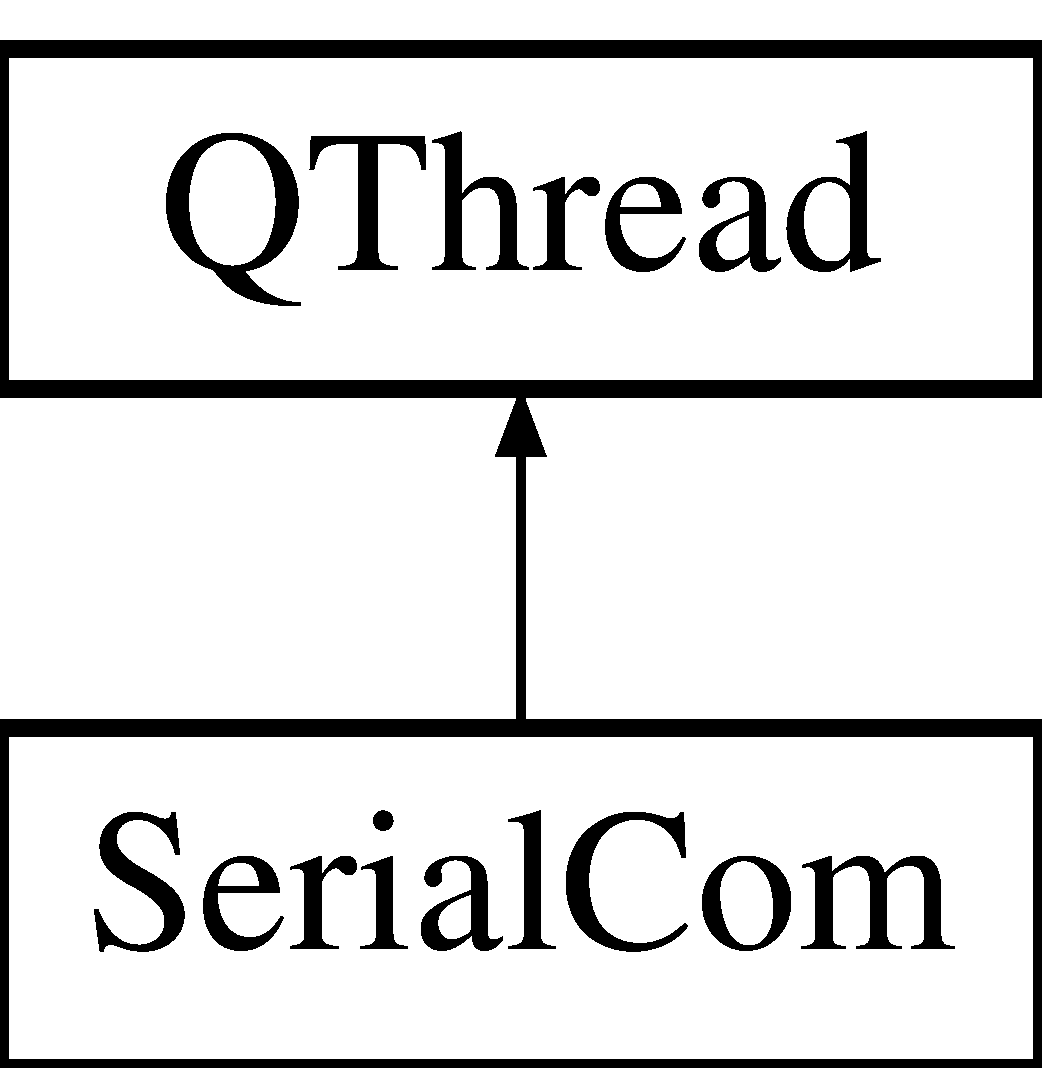
\includegraphics[height=2.000000cm]{class_serial_com}
\end{center}
\end{figure}
\subsection*{Signals}
\begin{DoxyCompactItemize}
\item 
void \hyperlink{class_serial_com_a9e83e2b67a01ee9504719c4b11375635}{response} (const Q\-String \&s)
\item 
void \hyperlink{class_serial_com_a453c5249e7e171dcc3a32b722ccaec23}{error} (const Q\-String \&s)
\item 
void \hyperlink{class_serial_com_acac1f4d821122f430e06ad13b964974f}{timeout} (const Q\-String \&s)
\end{DoxyCompactItemize}
\subsection*{Public Member Functions}
\begin{DoxyCompactItemize}
\item 
\hyperlink{class_serial_com_ae84f828a2adf56b4a20365a4de438ab4}{Serial\-Com} (Q\-Object $\ast$parent=0)
\item 
\hyperlink{class_serial_com_a5582cf804e661a24cb32720b31a2f9fe}{$\sim$\-Serial\-Com} ()
\item 
void \hyperlink{class_serial_com_aeefa54d2e7de44116e9ee6178020607e}{send\-Request} (const Q\-String \&port, int wait\-Time, const Q\-String \&request)
\item 
void \hyperlink{class_serial_com_a842c52f3e42ee3cc4b7c1ebaff83c560}{run} ()
\end{DoxyCompactItemize}


\subsection{Detailed Description}
This class is used for funtions related to serial communication with the arduino. 

Definition at line 26 of file Serial\-Com.\-hpp.



\subsection{Constructor \& Destructor Documentation}
\hypertarget{class_serial_com_ae84f828a2adf56b4a20365a4de438ab4}{\index{Serial\-Com@{Serial\-Com}!Serial\-Com@{Serial\-Com}}
\index{Serial\-Com@{Serial\-Com}!SerialCom@{Serial\-Com}}
\subsubsection[{Serial\-Com}]{\setlength{\rightskip}{0pt plus 5cm}Q\-T\-\_\-\-U\-S\-E\-\_\-\-N\-A\-M\-E\-S\-P\-A\-C\-E Serial\-Com\-::\-Serial\-Com (
\begin{DoxyParamCaption}
\item[{Q\-Object $\ast$}]{parent = {\ttfamily 0}}
\end{DoxyParamCaption}
)}}\label{class_serial_com_ae84f828a2adf56b4a20365a4de438ab4}
Class constructor

Constructor\-: 

Definition at line 27 of file Serial\-Com.\-cpp.

\hypertarget{class_serial_com_a5582cf804e661a24cb32720b31a2f9fe}{\index{Serial\-Com@{Serial\-Com}!$\sim$\-Serial\-Com@{$\sim$\-Serial\-Com}}
\index{$\sim$\-Serial\-Com@{$\sim$\-Serial\-Com}!SerialCom@{Serial\-Com}}
\subsubsection[{$\sim$\-Serial\-Com}]{\setlength{\rightskip}{0pt plus 5cm}Serial\-Com\-::$\sim$\-Serial\-Com (
\begin{DoxyParamCaption}
{}
\end{DoxyParamCaption}
)}}\label{class_serial_com_a5582cf804e661a24cb32720b31a2f9fe}
Class destructor

Destructor\-: 

Definition at line 35 of file Serial\-Com.\-cpp.



\subsection{Member Function Documentation}
\hypertarget{class_serial_com_a453c5249e7e171dcc3a32b722ccaec23}{\index{Serial\-Com@{Serial\-Com}!error@{error}}
\index{error@{error}!SerialCom@{Serial\-Com}}
\subsubsection[{error}]{\setlength{\rightskip}{0pt plus 5cm}void Serial\-Com\-::error (
\begin{DoxyParamCaption}
\item[{const Q\-String \&}]{s}
\end{DoxyParamCaption}
)\hspace{0.3cm}{\ttfamily [signal]}}}\label{class_serial_com_a453c5249e7e171dcc3a32b722ccaec23}
Error from arduino \hypertarget{class_serial_com_a9e83e2b67a01ee9504719c4b11375635}{\index{Serial\-Com@{Serial\-Com}!response@{response}}
\index{response@{response}!SerialCom@{Serial\-Com}}
\subsubsection[{response}]{\setlength{\rightskip}{0pt plus 5cm}void Serial\-Com\-::response (
\begin{DoxyParamCaption}
\item[{const Q\-String \&}]{s}
\end{DoxyParamCaption}
)\hspace{0.3cm}{\ttfamily [signal]}}}\label{class_serial_com_a9e83e2b67a01ee9504719c4b11375635}
Response from the arduino \hypertarget{class_serial_com_a842c52f3e42ee3cc4b7c1ebaff83c560}{\index{Serial\-Com@{Serial\-Com}!run@{run}}
\index{run@{run}!SerialCom@{Serial\-Com}}
\subsubsection[{run}]{\setlength{\rightskip}{0pt plus 5cm}void Serial\-Com\-::run (
\begin{DoxyParamCaption}
{}
\end{DoxyParamCaption}
)}}\label{class_serial_com_a842c52f3e42ee3cc4b7c1ebaff83c560}
To send a request to arduino and wait for response and to save it

\hyperlink{class_serial_com_a842c52f3e42ee3cc4b7c1ebaff83c560}{run()} 

Definition at line 64 of file Serial\-Com.\-cpp.

\hypertarget{class_serial_com_aeefa54d2e7de44116e9ee6178020607e}{\index{Serial\-Com@{Serial\-Com}!send\-Request@{send\-Request}}
\index{send\-Request@{send\-Request}!SerialCom@{Serial\-Com}}
\subsubsection[{send\-Request}]{\setlength{\rightskip}{0pt plus 5cm}void Serial\-Com\-::send\-Request (
\begin{DoxyParamCaption}
\item[{const Q\-String \&}]{port, }
\item[{int}]{wait\-Time, }
\item[{const Q\-String \&}]{request}
\end{DoxyParamCaption}
)}}\label{class_serial_com_aeefa54d2e7de44116e9ee6178020607e}
To set the parameters that needed to sent to arduino 
\begin{DoxyParams}{Parameters}
{\em port} & name of the port on which request need to be sent \\
\hline
{\em wait\-Time} & wait time for the response from arduino \\
\hline
{\em request} & a string to be sent to arduino\\
\hline
\end{DoxyParams}
send\-Request(const Q\-String, int, const Q\-String)\-: Send a request to arduino 

Definition at line 48 of file Serial\-Com.\-cpp.

\hypertarget{class_serial_com_acac1f4d821122f430e06ad13b964974f}{\index{Serial\-Com@{Serial\-Com}!timeout@{timeout}}
\index{timeout@{timeout}!SerialCom@{Serial\-Com}}
\subsubsection[{timeout}]{\setlength{\rightskip}{0pt plus 5cm}void Serial\-Com\-::timeout (
\begin{DoxyParamCaption}
\item[{const Q\-String \&}]{s}
\end{DoxyParamCaption}
)\hspace{0.3cm}{\ttfamily [signal]}}}\label{class_serial_com_acac1f4d821122f430e06ad13b964974f}
Timeout error from arduio 

The documentation for this class was generated from the following files\-:\begin{DoxyCompactItemize}
\item 
\hyperlink{_serial_com_8hpp}{Serial\-Com.\-hpp}\item 
\hyperlink{_serial_com_8cpp}{Serial\-Com.\-cpp}\end{DoxyCompactItemize}

\chapter{File Documentation}
\hypertarget{_calibrate_8cpp}{\section{Calibrate.\-cpp File Reference}
\label{_calibrate_8cpp}\index{Calibrate.\-cpp@{Calibrate.\-cpp}}
}
{\ttfamily \#include \char`\"{}Calibrate.\-hpp\char`\"{}}\\*
{\ttfamily \#include $<$Q\-Media\-Player$>$}\\*
{\ttfamily \#include $<$Q\-Completer$>$}\\*
{\ttfamily \#include $<$Q\-File\-Dialog$>$}\\*
{\ttfamily \#include $<$Q\-File$>$}\\*
{\ttfamily \#include $<$Q\-Debug$>$}\\*
{\ttfamily \#include $<$Q\-Text\-Stream$>$}\\*
{\ttfamily \#include $<$Q\-Object$>$}\\*
{\ttfamily \#include $<$Q\-String$>$}\\*
{\ttfamily \#include $<$Q\-Time$>$}\\*
{\ttfamily \#include $<$Q\-Date\-Time$>$}\\*
{\ttfamily \#include $<$Q\-Message\-Box$>$}\\*
{\ttfamily \#include $<$Q\-Input\-Dialog$>$}\\*
{\ttfamily \#include $<$Q\-Exception$>$}\\*
{\ttfamily \#include $<$Q\-Reg\-Exp$>$}\\*
{\ttfamily \#include $<$Q\-Reg\-Exp\-Validator$>$}\\*
{\ttfamily \#include $<$Q\-List$>$}\\*
{\ttfamily \#include $<$Q\-Widget$>$}\\*
{\ttfamily \#include $<$Q\-Byte\-Array$>$}\\*
{\ttfamily \#include $<$Q\-Core\-Application$>$}\\*
{\ttfamily \#include $<$stdio.\-h$>$}\\*

\hypertarget{_calibrate_8hpp}{\section{Calibrate.\-hpp File Reference}
\label{_calibrate_8hpp}\index{Calibrate.\-hpp@{Calibrate.\-hpp}}
}
{\ttfamily \#include $<$math.\-h$>$}\\*
\subsection*{Classes}
\begin{DoxyCompactItemize}
\item 
class \hyperlink{class_calibrate}{Calibrate}
\begin{DoxyCompactList}\small\item\em Library for coordinates transformations. Calculates the equivalent coordinates between both coordinate systems equatorial and horizontal. \end{DoxyCompactList}\end{DoxyCompactItemize}

\hypertarget{_o_s_p_main_dialog_8cpp}{\section{gui/\-O\-S\-P\-Main\-Dialog.cpp File Reference}
\label{_o_s_p_main_dialog_8cpp}\index{gui/\-O\-S\-P\-Main\-Dialog.\-cpp@{gui/\-O\-S\-P\-Main\-Dialog.\-cpp}}
}
{\ttfamily \#include \char`\"{}Open\-Sky\-Planetarium.\-hpp\char`\"{}}\\*
{\ttfamily \#include \char`\"{}O\-S\-P\-Main\-Dialog.\-hpp\char`\"{}}\\*
{\ttfamily \#include \char`\"{}ui\-\_\-\-O\-S\-P\-Main\-Dialog.\-h\char`\"{}}\\*
{\ttfamily \#include \char`\"{}Calibrate.\-hpp\char`\"{}}\\*
{\ttfamily \#include \char`\"{}Stel\-App.\-hpp\char`\"{}}\\*
{\ttfamily \#include \char`\"{}Stel\-Locale\-Mgr.\-hpp\char`\"{}}\\*
{\ttfamily \#include \char`\"{}Stel\-Module.\-hpp\char`\"{}}\\*
{\ttfamily \#include \char`\"{}Stel\-Module\-Mgr.\-hpp\char`\"{}}\\*
{\ttfamily \#include \char`\"{}Stel\-Object\-Mgr.\-hpp\char`\"{}}\\*
{\ttfamily \#include \char`\"{}Stel\-Utils.\-hpp\char`\"{}}\\*
{\ttfamily \#include \char`\"{}Stel\-File\-Mgr.\-hpp\char`\"{}}\\*
{\ttfamily \#include \char`\"{}Star\-Mgr.\-hpp\char`\"{}}\\*
{\ttfamily \#include \char`\"{}Stel\-Audio\-Mgr.\-hpp\char`\"{}}\\*
{\ttfamily \#include $<$Q\-Media\-Player$>$}\\*
{\ttfamily \#include $<$Q\-Completer$>$}\\*
{\ttfamily \#include $<$Q\-File\-Dialog$>$}\\*
{\ttfamily \#include $<$Q\-File$>$}\\*
{\ttfamily \#include $<$Q\-Input\-Dialog$>$}\\*
{\ttfamily \#include $<$Q\-Exception$>$}\\*
{\ttfamily \#include $<$Q\-Reg\-Exp$>$}\\*
{\ttfamily \#include $<$Q\-Reg\-Exp\-Validator$>$}\\*
{\ttfamily \#include $<$Q\-List$>$}\\*
{\ttfamily \#include $<$Q\-Message\-Box$>$}\\*
{\ttfamily \#include $<$Q\-Widget$>$}\\*
{\ttfamily \#include $<$Q\-Byte\-Array$>$}\\*
{\ttfamily \#include $<$Q\-Date\-Time$>$}\\*
{\ttfamily \#include $<$Q\-Core\-Application$>$}\\*

\hypertarget{_o_s_p_main_dialog_8hpp}{\section{gui/\-O\-S\-P\-Main\-Dialog.hpp File Reference}
\label{_o_s_p_main_dialog_8hpp}\index{gui/\-O\-S\-P\-Main\-Dialog.\-hpp@{gui/\-O\-S\-P\-Main\-Dialog.\-hpp}}
}
{\ttfamily \#include \char`\"{}Calibrate.\-hpp\char`\"{}}\\*
{\ttfamily \#include \char`\"{}Stel\-Dialog.\-hpp\char`\"{}}\\*
{\ttfamily \#include \char`\"{}Laser\-Dev.\-hpp\char`\"{}}\\*
{\ttfamily \#include \char`\"{}Star\-Mgr.\-hpp\char`\"{}}\\*
{\ttfamily \#include $<$Q\-Media\-Player$>$}\\*
{\ttfamily \#include $<$Q\-Widget$>$}\\*
{\ttfamily \#include $<$Qt\-Serial\-Port/\-Q\-Serial\-Port$>$}\\*
{\ttfamily \#include $<$Qt\-Serial\-Port/\-Q\-Serial\-Port\-Info$>$}\\*
{\ttfamily \#include $<$Q\-List$>$}\\*
{\ttfamily \#include $<$Q\-Hash$>$}\\*
{\ttfamily \#include $<$Q\-Media\-Playlist$>$}\\*
{\ttfamily \#include $<$Q\-Abstract\-Slider$>$}\\*
\subsection*{Classes}
\begin{DoxyCompactItemize}
\item 
class \hyperlink{class_o_s_p_main_dialog}{O\-S\-P\-Main\-Dialog}
\begin{DoxyCompactList}\small\item\em This is the main class used in connecting all the signals to gui. \end{DoxyCompactList}\end{DoxyCompactItemize}

\hypertarget{_laser_dev_8cpp}{\section{Laser\-Dev.\-cpp File Reference}
\label{_laser_dev_8cpp}\index{Laser\-Dev.\-cpp@{Laser\-Dev.\-cpp}}
}
{\ttfamily \#include \char`\"{}Laser\-Dev.\-hpp\char`\"{}}\\*
{\ttfamily \#include $<$Qt\-Serial\-Port/\-Q\-Serial\-Port\-Info$>$}\\*
{\ttfamily \#include $<$Qt\-Serial\-Port/\-Q\-Serial\-Port$>$}\\*
{\ttfamily \#include $<$Q\-Core\-Application$>$}\\*
{\ttfamily \#include $<$Q\-Text\-Stream$>$}\\*
{\ttfamily \#include $<$Q\-Object$>$}\\*
{\ttfamily \#include $<$Q\-Debug$>$}\\*
{\ttfamily \#include $<$Q\-String$>$}\\*
{\ttfamily \#include $<$Q\-Time$>$}\\*
{\ttfamily \#include $<$Q\-Date\-Time$>$}\\*
{\ttfamily \#include $<$Q\-Message\-Box$>$}\\*
{\ttfamily \#include \char`\"{}Serial\-Com.\-hpp\char`\"{}}\\*

\hypertarget{_laser_dev_8hpp}{\section{Laser\-Dev.\-hpp File Reference}
\label{_laser_dev_8hpp}\index{Laser\-Dev.\-hpp@{Laser\-Dev.\-hpp}}
}
{\ttfamily \#include $<$Qt\-Serial\-Port/\-Q\-Serial\-Port\-Info$>$}\\*
{\ttfamily \#include $<$Qt\-Serial\-Port/\-Q\-Serial\-Port$>$}\\*
{\ttfamily \#include $<$Q\-Text\-Stream$>$}\\*
{\ttfamily \#include $<$Q\-Core\-Application$>$}\\*
{\ttfamily \#include $<$Q\-String$>$}\\*
{\ttfamily \#include $<$Q\-Object$>$}\\*
{\ttfamily \#include $<$Q\-Thread$>$}\\*
{\ttfamily \#include $<$Q\-Time$>$}\\*
{\ttfamily \#include \char`\"{}Serial\-Com.\-hpp\char`\"{}}\\*
\subsection*{Classes}
\begin{DoxyCompactItemize}
\item 
class \hyperlink{class_laser_dev}{Laser\-Dev}
\begin{DoxyCompactList}\small\item\em This class is used for funtions related to motion and turning the laser on and off. \end{DoxyCompactList}\end{DoxyCompactItemize}

\hypertarget{_open_sky_planetarium_8cpp}{\section{Open\-Sky\-Planetarium.\-cpp File Reference}
\label{_open_sky_planetarium_8cpp}\index{Open\-Sky\-Planetarium.\-cpp@{Open\-Sky\-Planetarium.\-cpp}}
}
{\ttfamily \#include \char`\"{}Stel\-App.\-hpp\char`\"{}}\\*
{\ttfamily \#include \char`\"{}Stel\-Core.\-hpp\char`\"{}}\\*
{\ttfamily \#include \char`\"{}Stel\-Locale\-Mgr.\-hpp\char`\"{}}\\*
{\ttfamily \#include \char`\"{}Stel\-Module\-Mgr.\-hpp\char`\"{}}\\*
{\ttfamily \#include \char`\"{}Stel\-Gui.\-hpp\char`\"{}}\\*
{\ttfamily \#include \char`\"{}Stel\-Gui\-Items.\-hpp\char`\"{}}\\*
{\ttfamily \#include \char`\"{}Open\-Sky\-Planetarium.\-hpp\char`\"{}}\\*
{\ttfamily \#include \char`\"{}O\-S\-P\-Main\-Dialog.\-hpp\char`\"{}}\\*
{\ttfamily \#include $<$Q\-Action$>$}\\*
{\ttfamily \#include $<$Q\-String$>$}\\*
{\ttfamily \#include $<$Q\-Debug$>$}\\*
{\ttfamily \#include $<$stdexcept$>$}\\*

\hypertarget{_open_sky_planetarium_8hpp}{\section{Open\-Sky\-Planetarium.\-hpp File Reference}
\label{_open_sky_planetarium_8hpp}\index{Open\-Sky\-Planetarium.\-hpp@{Open\-Sky\-Planetarium.\-hpp}}
}
{\ttfamily \#include \char`\"{}Stel\-Module.\-hpp\char`\"{}}\\*
{\ttfamily \#include \char`\"{}Stel\-Gui.\-hpp\char`\"{}}\\*
{\ttfamily \#include $<$Q\-String$>$}\\*
{\ttfamily \#include $<$Q\-Font$>$}\\*
{\ttfamily \#include $<$Q\-Object$>$}\\*
{\ttfamily \#include \char`\"{}Stel\-Plugin\-Interface.\-hpp\char`\"{}}\\*
\subsection*{Classes}
\begin{DoxyCompactItemize}
\item 
class \hyperlink{class_open_sky_planetarium}{Open\-Sky\-Planetarium}
\begin{DoxyCompactList}\small\item\em This is used to dynamically load Open Sky Planetarium plugin into stellarium. \end{DoxyCompactList}\item 
class \hyperlink{class_open_sky_planetarium_plugin_interface}{Open\-Sky\-Planetarium\-Plugin\-Interface}
\begin{DoxyCompactList}\small\item\em This class is used by Qt to manage a plug-\/in interface. \end{DoxyCompactList}\end{DoxyCompactItemize}

\hypertarget{_serial_com_8cpp}{\section{Serial\-Com.\-cpp File Reference}
\label{_serial_com_8cpp}\index{Serial\-Com.\-cpp@{Serial\-Com.\-cpp}}
}
{\ttfamily \#include \char`\"{}Serial\-Com.\-hpp\char`\"{}}\\*
{\ttfamily \#include $<$Qt\-Serial\-Port/\-Q\-Serial\-Port$>$}\\*
{\ttfamily \#include $<$Q\-Time$>$}\\*

\hypertarget{_serial_com_8hpp}{\section{Serial\-Com.\-hpp File Reference}
\label{_serial_com_8hpp}\index{Serial\-Com.\-hpp@{Serial\-Com.\-hpp}}
}
{\ttfamily \#include $<$Q\-Thread$>$}\\*
{\ttfamily \#include $<$Q\-Mutex$>$}\\*
{\ttfamily \#include $<$Q\-Wait\-Condition$>$}\\*
\subsection*{Classes}
\begin{DoxyCompactItemize}
\item 
class \hyperlink{class_serial_com}{Serial\-Com}
\begin{DoxyCompactList}\small\item\em This class is used for funtions related to serial communication with the arduino. \end{DoxyCompactList}\end{DoxyCompactItemize}

%--- End generated contents ---

% Index
\newpage
\phantomsection
\addcontentsline{toc}{chapter}{Index}
\printindex

\end{document}
